\documentclass[a4paper,10pt,oneside]{article}
\usepackage[top=2cm,bottom=2cm,left=1cm,right=1cm]{geometry}
%\usepackage{fontspec}
\usepackage[utf8]{inputenc}
\usepackage{hyperref}
\usepackage{enumitem}
\usepackage{changepage}
\usepackage[table]{xcolor}
\usepackage{graphicx}
\usepackage{fancyhdr}
\pagestyle{fancy}
\usepackage{titlesec}
\usepackage{longtable}
\usepackage{setspace}
\usepackage{amsmath}
\usepackage{xcolor}
\usepackage{listings}


\hypersetup{
	colorlinks=true,      
	urlcolor=magenta,
	linkcolor  = black
}

\definecolor{mGreen}{rgb}{0,0.6,0}
\definecolor{mGray}{rgb}{0.5,0.5,0.5}
\definecolor{mPurple}{rgb}{0.58,0,0.82}
\definecolor{backgroundColour}{rgb}{0.95,0.95,0.92}

\lstdefinestyle{CStyle}{
	backgroundcolor=\color{backgroundColour},   
	commentstyle=\color{mGreen},
	keywordstyle=\color{magenta},
	numberstyle=\tiny\color{mGray},
	stringstyle=\color{mPurple},
	basicstyle=\footnotesize,
	breakatwhitespace=false,         
	breaklines=true,                 
	captionpos=b,                    
	keepspaces=true,                 
	numbers=left,                    
	numbersep=5pt,                  
	showspaces=false,                
	showstringspaces=false,
	showtabs=false,                  
	tabsize=2,
	language=C
}

\title{\Huge{\textbf{Tiva Based Daughter Board for Firebird V \\ Hardware And Software Manual.}}}

\author{\textbf{ eRTS Lab IIT Bombay}}

\rhead{Manual for Tiva Based Daughter Board for Firebird V.}
\lfoot{eRTS Lab IIT Bombay}

\renewcommand*\contentsname{\Huge \textbf{Table Of Content}}

\setcounter{secnumdepth}{4}

\titleformat{\paragraph}
{\normalfont\normalsize\bfseries}{\theparagraph}{1em}{}
\titlespacing*{\paragraph}
{0pt}{3.25ex plus 1ex minus .2ex}{1.5ex plus .2ex}

\begin{document}
	\large
	\maketitle
	\newpage
	\section{\Huge{\textbf{Credits}}}
	\textbf{\\\\ Version 1.0\\\date{\today}}% Right allign
	\\
	\\
	\\
	\\
	{\large{\textbf{Documentation Author(Alphabetical Order):}
			\begin{enumerate}
			\item Ayush Gaurav, Intern eYSIP 2017
			\item Nagesh K,  Intern eYSIP 2017
	\end{enumerate}
	\textbf{Credits(Alphabetical Order):}
		\begin{enumerate}
			\item Prof Kavi Arya, CSE IIT Bombay
			\item Nex Robotics Pvt. Ltd.
			\item Piyush Manavar, Team e-Yantra
			\item Saurav Shandilya, Team e-Yantra
	\end{enumerate}}
	\newpage
	\section{\Huge{\textbf{Notice}}}
	{\large The contents of this manual are subject to change without notice. All efforts have been made to
	ensure the accuracy of contents in this manual. However, should any errors be detected, e-yantra welcomes your corrections. You can send us your queries / suggestions at
	\href{mailto:helpdesk@eyantra.org}{Contact Us}\\}
	\newpage
	\doublespacing
	\tableofcontents
	\singlespacing
	\newpage 
	\section{\Huge\textbf{Introduction}}
	Tiva Daughter board for Fire Bird V will help you gain exposure to the world of robotics and embedded systems with ARM Cortex M4. The board is designed with Open Source Philosophy in software and hardware design ,you will be able to create and contribute to complex applications that run on this platform, helping you	acquire expertise as you spend more time with them.
	\subsection{\textbf{Safety precautions:}}
	\begin{itemize}

	\item  Robot’s electronics is static sensitive. Use robot in static free environment.
	\item Read the assembling and operating instructions before working with the robot.
	\item If robot’s battery low buzzer starts beeping, immediately charge the batteries.
	\item To prevent fire hazard, do not expose the equipment to rain or moisture.
	\item Refrain from dismantling the unit or any of its accessories once robot is assembled.
	\item Charge the NiMH battery only with the charger provided on the robot.
	\item Never allow NiMH battery to deep discharge.
	\item Mount all the components with correct polarity.
	\item Keep wheels away from long hair or fur.
	\item Keep the robot away from the wet areas. Contact with water will damage the robot.
	\item To avoid risk of fall, keep your robot in a stable position.
	\item Do not attach any connectors while robot is powered ON.
	\item Never leave the robot powered ON when it is not in use.
	\item Disconnect the battery charger after charging the robot. 
\end{itemize}
	\subsection{\textbf{Inappropriate Operation:}}
	Inappropriate operation can damage your robot. Inappropriate operation includes, but is not
	limited to:
	\begin{itemize}
	\item Dropping the robot, running it off an edge, or otherwise operating it in irresponsible
	manner.
	\item Interfacing new hardware without considering compatibility.
	\item Overloading the robot above its payload capacity.
	\item Exposing the robot to wet environments.
	\item Continuing to run the robot after hair, yarn, string, or any other item is entangled in the
	robot’s axles or wheels.
	\item All other forms of inappropriate operations.
	\item Using robot in areas prone to static electricity.
	\item Read carefully paragraphs marked with caution symbol.
	\end{itemize}
	\section{\Huge\textbf{Tiva Based Daughter Board}}
		{There are two daughter boards one with the launchpad and other one with the Arm Cortex M4 based uC. Almost all the specification are same unless mentioned otherwise.\\}
		\subsection{{\huge \textbf{Technical Specification}}\\}
			{\textbf{Microcontroller:\\}
			TM4C123gh6pm (ARM architecture based Microcontroller)\\ To know more about the microcontroller please refer to \href{www.ti.com/lit/gpn/tm4c123gh6pm}{datasheet}.\\ \\}
			{\textbf{Sensors:}\\
			Three white line sensors (extendable to 7)\\
			Five Sharp GP2Y0A02YK IR range sensor (One in default configuration)\\
			Eight analog IR proximity sensors\\
			Two position encoders\\\\} 
			\textbf{Indicators:\\}
			{2 x 16 Characters LCD\\
			Buzzer\\\\}
			\textbf{Communication:\\}
			{USB Communication\\
			Wireless ZigBee Communication (2.4GHZ) (if XBee wireless module is installed)\\
			Bluetooth communication(Can be interfaced on external UART0 available on the board)\\
			Simplex infrared communication (From infrared remote to robot)\\
			I2C Communication \\\\}
			\textbf{Battery Life:\\}
			{2 Hours, while motors are operational at 75\% of time\\\\}
			\textbf{Locomotion:\\}
			{Two DC geared motors in differential drive configuration and caster wheel at front as support\\
			Top Speed: 24 cm / second\\
			Wheel Diameter: 51mm\\
			Position encoder: 30 pulses per revolution\\
			Position encoder resolution: 5.44 mm\\\\}
		%\subsection{}%start with the functionality
	\section{\Huge\textbf{Hardware Manual:}}
	%mention about the upcoming sub section in brief
	\subsection{\huge \textbf{Voltage Regulation on the Daughter Board\\}}
	{The voltage source available on the Firebird is 9.6V. But the TIVA platform works on 3.3V and the servos can operate upto 6V. So there must be 3 different voltage levels on the board. The uC based board has 2 voltage regulators and the plug and play board has 1 voltage regulator. In the uC based board the 9.6 volts is 3.3V to power the microcontroller. In the plug and play board the there is an inbuilt voltage regulator, so it is directly connected connected to 5v, 300mA source. The servo in both the boards has a separate 5V regulator.}
	
	\subsubsection{\Large \textbf{Powering Micro-controller}}
	{The boards have different powering circuits.In the plug and play board is connected to 5V source on Pin 10. In the uC based board the 9.6V source available on Pin 29 is reduced to 3.3V. Refer to the schematic below for further details.\\} 
				
	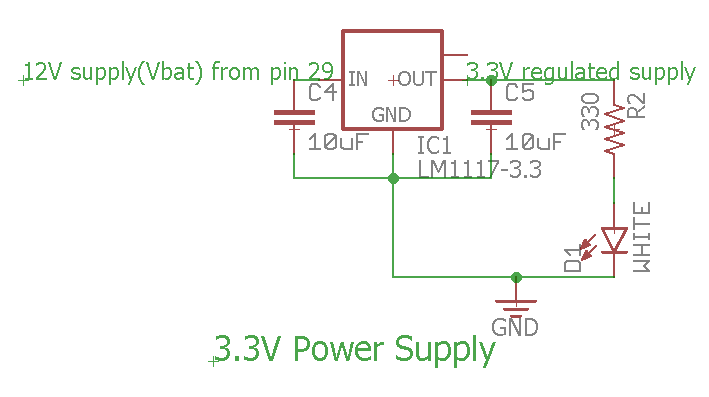
\includegraphics[width=18cm, height=8cm]{3VPowerSupply}\\\\
				
	\subsubsection{\Large \textbf{Powering Servos}}
	{The servo motors can operate safely up to 6V, beyond this voltage they get damaged. Also, the servos require high current. There is a separate power line for servos taken from Pin 29 and reduced to 5V using the voltage regulator. Refer the schematic for further details.\\ }
		
	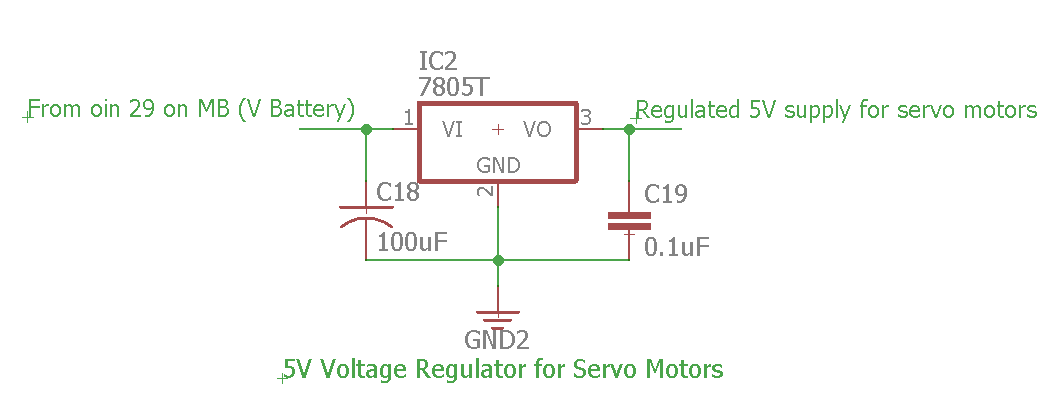
\includegraphics[width=18cm, height=8cm]{ServoPowerSupply}\\			
	\subsection{\huge \textbf{Level Converters}}
	{The TIVA platform operates at 3.3V and the Firebird operates at 5V. Directly connecting these pins to the TIVA may be fatal. So to interface these sensors, a level converter is used. A bidirectional MOSFET based level converter used. The level converter is necessary is for input pins. In the boards Level converter is used for interfacing the position encoders of the motors. Refer the schematic for further details.\\ }
		
	\hspace{3.5cm}
	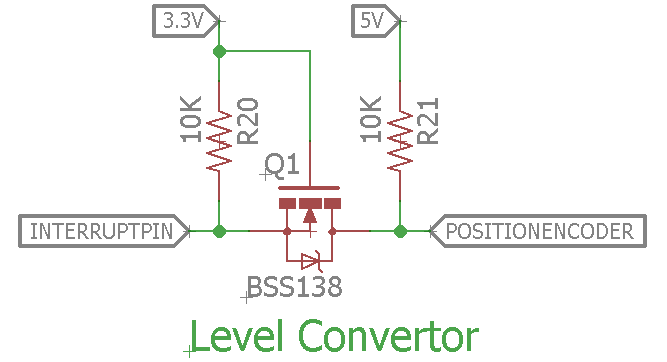
\includegraphics[width=12cm, height=6cm]{Level_Converter}\\
	\begin{tabular}{|c|}
		\hline
		\\
		\textbf{NOTE: If the user wishes to interface extra sensors using the GPIOs provided on the board,} \\ \textbf{then external level converters have to used if the output of the sensor is above 3.3V.}
		\\
		\hline
	\end{tabular}\\\\
	\subsection{\huge \textbf{Sensors}}{The firebird V has as many as 22 sensors, but maximum 12 sensors can be interfaced directly with the controller. The daughter board has interfaced 20 of those 22 sensors using external I2C bases ADC. Sensors that were not included in the daughter board are current sensor and battery monitoring sensor. These sensors are working either on 3.3V or on 5V. Interfacing 3.3V sensors are simple and can be directly connected to the controller. On the other hand 5V can not be directly interfaced so a different approach is taken which will be mentioned in the 5V sensors sub heading.}
		\subsubsection{\Large \textbf{3.3V sensors}}
		{The output white line sensors and IR Proximity sensors vary from 0  to 3.3V. Hence these sensors can be interfaced directly with the microcontroller. Refer the table below for pin connections.\\
		\begin{center}
		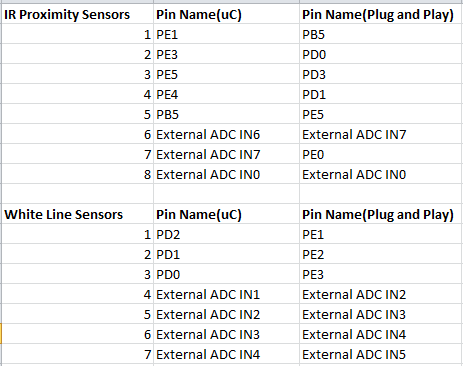
\includegraphics{3v3Sensors}\\
		\end{center}
	}
		\subsubsection{\Large \textbf{5V sensors}}
		{Sharp Sensors are the only sensors on board that works on 5V supply. The output of the sharp sensor ranges from 0-5V and according to the output we have a formula to calculate the distance. While uC has VREF as 3.3V so these sensors cannot be directly connected. The approach we followed is to feed the output of the sensor to a buffer and then using a voltage divider convert 0-5 range to 0-3V range. For better understanding refer to the schematic below. There is a  also table which tells about the pin connection.}
		\begin{center}
			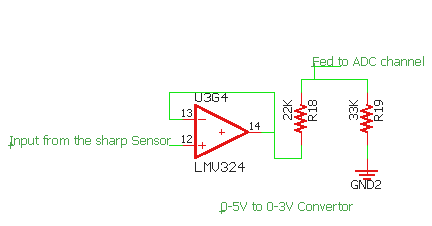
\includegraphics{5Vsensor1}\\
			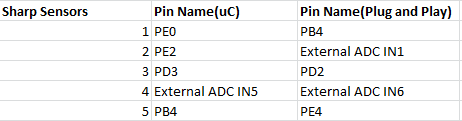
\includegraphics{5Vsensor2}\\
		\end{center}
	\subsection{\huge \textbf{Port Expander}}
	{TM4C123GH6PM has only 64 pins out which only 43 are GPIO pins. This limits our application to read input and respond correspondingly. To increase the number of GPIO and there interrupts we have used I2C compatible a port expander MCP23017. It has 2 PORTS A and B, with each port having 8 Pins.The interrupts on each pin can also be monitored. To read more about it, download the datasheet from   \href{www.microchip.com/downloads/en/DeviceDoc/21952b.pdf}{here.}The schematic of the connection is shown below.Keep in mind that I2C SCL and SDA have already been pulled up using 10K resistor.\\}
	\begin{center}
		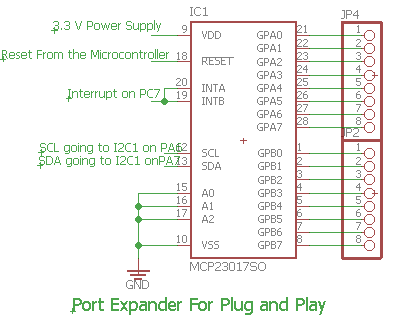
\includegraphics{portexpandePlug}\\
		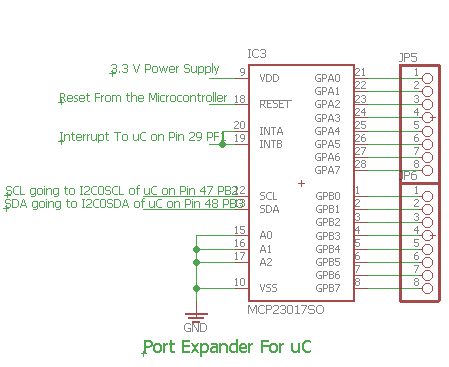
\includegraphics{portExpanderuc}\\
		\end{center}
	\subsection{\huge \textbf{External ADC}}
	{It has already been mentioned that adc channels on the microcontroller is limited to 12 while firebird has 22 sensors available. We have interfaced an external ADC which is also I2C compatible. It has  8 channel with 12 bit resolution.To read more about it, download the datasheet from \href{www.ti.com/lit/pdf/snas483}{here.}The schematic of the connection is shown below.Keep in mind that I2C SCL and SDA have already been pulled up using 10K resistor.\\}
		\begin{center}
		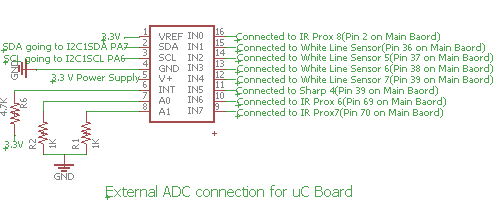
\includegraphics{externaladcuC}\\
		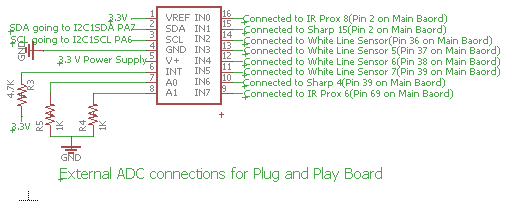
\includegraphics{externalADCplug}\\
	\end{center}
	\subsection{\huge \textbf{LCD Interfacing}}{
	LCD can be interfaced in 8bit or 4 bit interfacing mode. In 8 bit mode it requires 3 control line
	and 8 data lines. To reduce number of I/Os required, Fire Bird V robot uses 4 bit interfacing
	mode which requires 2 control lines and 4 data lines. In this mode upper and lower nibble of the
	data/command byte needs to be sent separately. RW(Read/Write) control line of lcd is grounded so it can only work in write mode.\\
	The EN line is used to tell the LCD that microcontroller
	has sent data to it or microcontroller is ready to receive data from LCD. This is indicated by a
	high-to-low transition on this line. To send data to the LCD, program should make sure that this
	line is low (0) and then set the other two control lines as required and put data on the data bus.
	When this is done, make EN high (1) and wait for the minimum amount of time as specified by
	the LCD datasheet, and end by bringing it to low (0) again.\\
	When RS is low (0), data is treated as a command or special
	instruction by the LCD (such as clear screen, position cursor, etc.). When RS is high (1), data
	being sent is treated as text data which should be displayed on the screen.\\
	written to the LCD.//}
		\begin{center}
		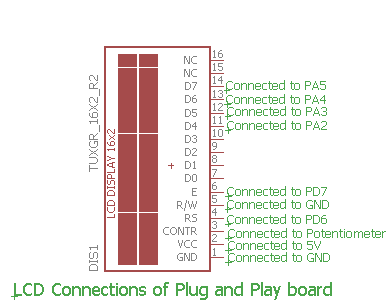
\includegraphics{lcdPlug}\\
		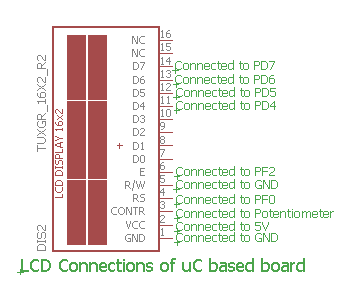
\includegraphics{lcduC}\\
		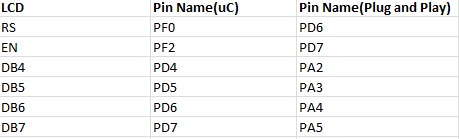
\includegraphics{lcdpin}
		\end{center}
	\subsection{\huge \textbf{USB Communication}}
	{Fire Bird V’s main board has USB port socket. Microcontroller accesses USB port via main
		board socket. All its pins are connected to the microcontroller adapter board via main board's
		socket connector.FT232 is a USB to TTL level serial converter. It is used for adding USB connectivity to the
		microcontroller adapter board. With onboard USB circuit Fire Bird V can communicate serially
		with the PC through USB port without the use of any external USB to Serial converter.
		Microcontroller socket uses USB port from the main board. Data transmission and reception is
		indicated suing TX and RX LEDs which are located near the FT232 IC. This IC is only on the uC based board. Plug and play board has its own usb port on TIVA launcpad. The schematic of ft232 is shown below.}
		\begin{center}
		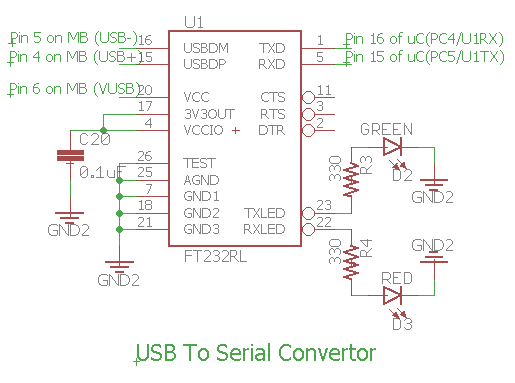
\includegraphics{ft232}\\
		\end{center}
	\subsection{\huge \textbf{Programing the Controller}}
	\subsection{\huge \textbf{Reset Switch}}
	{The Plug and play board makes use of reset button present on the TIVA launchpad. The uC based has a switch connected to the reset the reset pin 38 of the microcontroller. The schematic is given below.}\\
	\begin{center}
	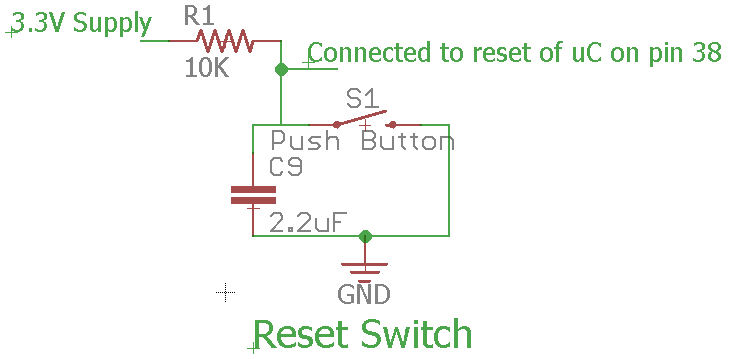
\includegraphics[width=13cm, height=6cm]{Reset_Switch}
	\end{center}
	\subsection{\huge \textbf{Servo Connectors}}
	{The microcontroller board has three Servo connectors. It can be used for
		driving servo motors of camera pod or any other attachment. Power for the servo connector is
		provided by the “5V servo supply” voltage regulator. Both the board have different pwm pins for servo which can be seen from the schematic. \\}
		\begin{center}
			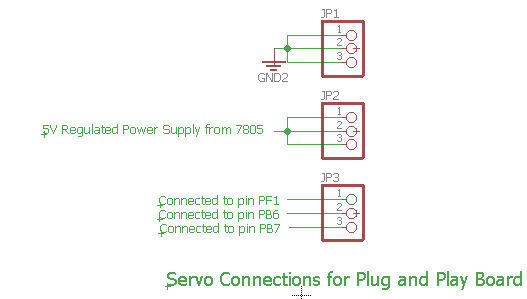
\includegraphics{servoPlug}\\
			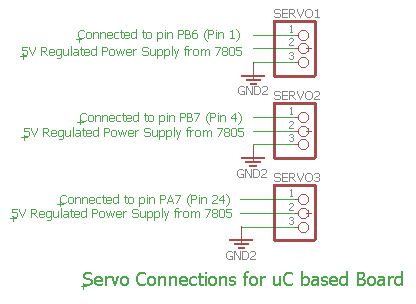
\includegraphics{servouc}\\
		\end{center}
	\subsection{\huge \textbf{TM4C123GH6PM Micro-controller:}}
	{The Tiva™ C Series ARM Cortex-M4 microcontrollers provide top performance and advanced
		integration. The product family is positioned for cost-conscious applications requiring significant
		control processing and connectivity capabilities such as:
		\begin{itemize}
		\item Low power, hand-held smart devices
		\item Gaming equipment
		\item Home and commercial site monitoring and control
		\item Motion control
		\item Medical instrumentation
		\item Test and measurement equipment
		\item	Factory automation
		\item Fire and security
		\item  Smart Energy/Smart Grid solutions
		\item Intelligent lighting control
		\item Transportation
	\end{itemize}
	Schematic Of the connections is shown below.}
	\begin{center}
		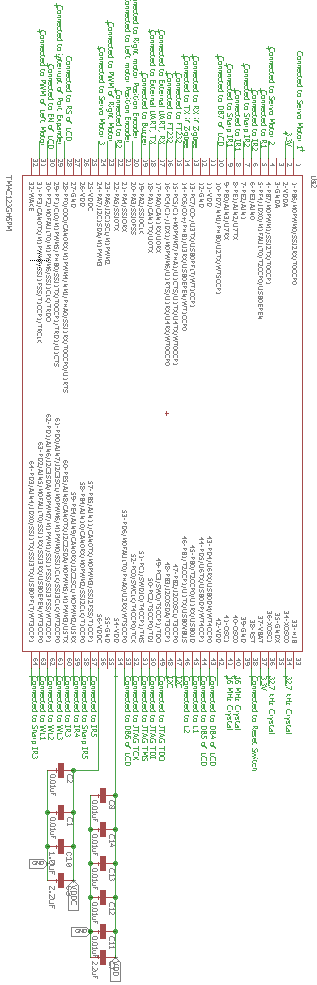
\includegraphics{uc}\\
	\end{center}
	\subsection{\huge \textbf{Pin Functionality}}
		\subsubsection{\Large\textbf{Pin of uC}}
			\begin{longtable}{|c|c|c|}\hline
				Pin No.&Pin & 	Complete Pin Connections\\ \hline
				1 &		PB6	&	Servo Motor 1\\ \hline
				2 &		VDDA&	VDD filtered through capcitors\\ \hline
				3 &		GNDA&	Ground\\ \hline
				4 &		PB7 &	Servo Motor 2\\ \hline
				5 & 	PF4 &	Pin 53 Right Motor 1\\ \hline
				6 &		PE3	&	16 IR proximity Sensor 2\\ \hline
				7 &		PE2 &	Output of Second OpAmp of lm324\\ \hline
				8 &		PE1 &	12 IR Proximity Sensor 1 \\ \hline
				9 &		PE0 &	output of First OpAmp of lm324\\ \hline
				10 &	PD7 &	28 DB7 of LCD Data\\ \hline
				11 &	VDD &	VDD filtered through capcitors\\ \hline
				12 &	GND	 &	Ground\\ \hline
				13 &	PC7	 &	13 Zigbee Rx\\ \hline
				14 &	PC6	 &	14 Zigbee Tx\\ \hline
				15 & 	PC5	 &	FT232\\ \hline
				16 & 	PC4 &	FT232\\ \hline 
				17 &	PA0 &	External UART\\ \hline
				18 &	PA1 &	External UART\\ \hline
				19 &	PA2 &	Buzzer\\ \hline
				20 &	PA3 &	63 Right Position Encoder Interrupt\\ \hline
				21 &	PA4	 &	64 Left Position Encoder Interrupt\\ \hline
				22 &	PA5 &	55 Right Motor 2\\ \hline
				23 &	PA6 &	54 Right Motor Pwm\\ \hline
				24 &	PA7 &	Servo Motor 3\\ \hline
				25 &	VDDC &	Connected to VDDC on 56\\ \hline
				26 &	VDD	 &	VDD filtered through capcitors\\ \hline
				27 &	GND	 &	Ground\\ \hline
				28 &	PF0	 &	22 RS of LCD\\ \hline
				29 &	PF1	 &	INT A and B of to GPIO expander shorted and connected\\ \hline
				30 &	PF2 &	24 EN of LCD\\ \hline
				31 &	PF3	 &	50 Left Motor PWM\\ \hline
				32 &	WAKE &	Ground\\ \hline
				33 &	HIB &	NC\\ \hline
				34 &	XOSC0 &	32.7 KHz crystals(One End)\\ \hline
				35 &	GNDX &	Cap to crystal\\ \hline
				36 &	XOSC1 &	32.7 KHz crystals(Other End)\\  \hline
				37 &	VBAT &	3.3 Volts\\ \hline
				38 &	RST	 &	Reset Switch\\ \hline
				39 &	GND	 &	Ground\\ \hline
				40 &	OSC1 &	16 MHz crystal(One end)\\ \hline
				41 &	OSC1 &	16 MHz crystal(Other end)\\ \hline
				42 &	VDD	 &	VDD filtered through capcitors\\ \hline
				43 &	PD4	 &	26 DB4 Of LCD \\ \hline
				44 &	PD5	 &	25 DB5 of LCD\\ \hline
				45 &	PB0	 &	51 Left Motor 1\\ \hline
				46 &	PB1	 &	52 Left Motor 2\\ \hline
				47 &	PB2	 &	I2C ADC SCL\\ \hline 
				48 &	PB3	 &	I2C ADC SDA\\ \hline
				49 &	PC3	 &	JTAG TDO\\ \hline
				50 &	PC2	 &	JTAG TDI\\ \hline
				51 &	PC1	 &	JTAG TMS\\ \hline
				52 &	PC0	 &	JTAG TCK\\ \hline
				53 &	PD6	 &	27 DB6 Of LCD\\ \hline
				54 &	VDD	 &	VDD filtered through capcitors\\ \hline
				55 &	GND	 &	Ground\\ \hline
				56 &	VDDC &	Connected to VDDC on 25\\ \hline
				57 &	PB5	 &	46 IR Proximity Sensor 5\\ \hline
				58 &	PB4	 &	Output of First OpAmp of lm358\\ \hline
				59 &	PE4	 &	43 IR Proximity Sensor 4\\ \hline
				60 &	PE5	 &	42 IR Proximity Sensor 3\\ \hline
				61 &	PD0	 &	32 White Line Sensor 3\\ \hline
				62 &	PD1	 &	31 White Line Sensor 2\\ \hline
				63 &	PD2	 &	30 White Line Sensor 1\\ \hline
				64 &	PD3	 &	Output of Third OpAmp of lm324\\ \hline
			\end{longtable}
		\subsubsection{\Large\textbf{Robot Main Board Connections}}
			\begin{longtable}{|p{.04\textwidth}|p{.25\textwidth}|p{.40\textwidth}|p{.1\textwidth}|p{.1\textwidth}|}\hline
				Pin Out&	Pin Name&	Functionality&	PIN on DB& Pin on Pluggable B\\ \hline
				1&	Current sensor&	Current sense analog value&	Not Using\\ \hline
				2&	IR Proximity sensor 8&	IR Proximity sensor 8 analog value&	External Adc INT0\\ \hline
				3&	GND&	Ground	&Ground\\ \hline
				4&	DATA+&	USB connection going to the ATMEGA2560	USB connection with uC & C4\\ \hline
				5&	DATA-&	microcontroller via FT232 USB to serial	USB connection with uC &PC5\\ \hline
				6&	VCC& USB	converter.	Connect TO VCC of FT232&\\ \hline
				7&	5V System&	"5V System Voltage. Can be used for powering
				up any digital device with current limit of
				400mA."	&\\ \hline
				8&	5V System&	"5V System Voltage. Can be used for powering
				up any digital device with current limit of
				300mA."	&\\ \hline
				9&	5V System&	"5V System Voltage. Can be used for powering
				up any digital device with current limit of
				300mA."	&\\ \hline
				10&	5V System&	"5V System Voltage. Can be used for powering
				up any digital device with current limit of
				400mA."	&\\ \hline
				11&	SHARP IR Range Sensor 1	&Analog output of Sharp IR range Sensor 1&	PE0(lm324 1)\\ \hline
				12&	IR Proximity Sensor 1&	Analog output of IR Proximity sensor 1&	PE1\\ \hline
				13&	XBee RXD&	XBee wireless module Serial data in	&PC7\\ \hline
				14&	XBee TXD&	XBee wireless module Serial data out&	PC6\\ \hline
				15&	SHARP IR Range Sensor 2	& Analog output of Sharp IR range sensor 2&	PE2(lm324 2)\\ \hline
				16&	IR Proximity Sensor 2&	Analog output of IR Proximity sensor 2&	PE3\\ \hline
				17&	RSSI&	To capture the RSSI signal&\\ \hline	
				18&	MOSI&	MOSI of the Controller/NC create extra expansion headers&\\ \hline	
				19&	MISO&	MISO of controller/NC create extra expansion headers	&\\ \hline
				20&	SCK&	SCK of the controller/NC create extra expansion headers&	\\ \hline
				21&	SSI	&SS of the controller/ NC create extra expansion headers	&\\ \hline
				22&	RS&	connected to RS of LCD normal I/O&	PF0\\ \hline
				23&	RW&	connected to RW of LCD normal I/O&	GND\\ \hline
				24&	EN&	connected to EN of LCD normal I/O&	PF2\\ \hline
				25&	DB5	&data pin of lcd normal I/O	&PD5\\ \hline
				26&	DB4&	data pin of lcd normal I/O&	PD4\\ \hline
				27&	DB6	&data pin of lcd normal I/O	&PD6\\ \hline
				28&	DB7	&data pin of lcd normal I/O	&PD7\\ \hline
				29&	V Battery System&	ADC to check the level of battery voltage	&\\ \hline
				30&	WL1&	Analog output of white line sensor 1	&PD2\\ \hline
				31&	WL2&	Analog output of white line sensor 2&	PD1\\ \hline
				32&	WL3&	Analog output of white line sensor 3&	PD0\\ \hline
				33&	"Sharp IR Sensors 1and 5
				Disable"& &		\\ \hline
				34&	IR Proximity Sensor Disable& &	\\ \hline	
				35&	5V System&	"5V system Voltage. Can be used for powering&
				up any digital device. Current Limit: 400mA."\\ \hline
				36&	WL4&	Analog output of white line sensor 4&	External Adc INT1\\ \hline
				37&	WL5&	Analog output of white line sensor 5&	External Adc INT2\\ \hline
				38&	WL6&	Analog output of white line sensor 6	&External Adc INT3\\ \hline
				39&	WL7&	Analog output of white line sensor 7&	External Adc INT4\\ \hline
				40&	White Line Sensors Disable&&\\ \hline		
				41&	Sharp IR Range Finder 3&	Analog output of Sharp IR range sensor 3	&PD3 (lm 324 3)\\ \hline
				42&	IR Proximity Sensor 3&	Analog output of IR Proximity sensor 3	&PE5\\ \hline
				43&	IR Proximity Sensor 4&	Analog output of IR Proximity sensor 4&	PE4\\ \hline
				44&	Sharp IR Range Finder 4	&Analog output of Sharp IR range sensor 4&	in 5 ex (lm 324 5)\\ \hline
				45&	Sharp IR Range Finder 5&	Analog output of Sharp IR range sensor 5&	PB4 (lm358 1)\\ \hline
				46&	IR Proximity Sensor 5&	Analog output of IR Proximity sensor 5&	PB5\\ \hline
				47&	C11& motor 	not present&	\\ \hline
				48&	C1 &PWM	not present	&\\ \hline
				49&	c12&	not present	&\\ \hline
				50&	PWM L&	left motor PWM(timer pin in PWM mode)&	PF3\\ \hline
				51&	L1&	left motor pin1 normal I/O&	PB0\\ \hline
				52&	L2&	left motor pin2 normal I/O&	PB1\\ \hline
				53&	R1&	right motor pin1 normal I/O&	PF4\\ \hline
				54&	PWM R2&	right motor PWM(timer pin in PWM  mode)&	PA6\\ \hline
				55&	R2&	right motor pin2&	PA5\\ \hline
				56&	NC&&	\\ \hline	
				57&	NC&&	\\ \hline	
				58&	NC&&	\\ \hline	
				59&	NC&&	\\ \hline	
				60&	NC&&	\\ \hline	
				61&	NC	&&	\\ \hline
				62&	Position encoder left&	Output of Left position encoder (0-5V)	PA4&&\\ \hline
				63&	Position encoder right& 	Output of Right position encoder (0-5V)	PA3&&\\ \hline
				64&	position enocder C2&	Output of C2 position encoder (0-5V)&&	\\ \hline
				65&	Position encoder C1& Output of C1 position encoder (0-5V)&&	\\ \hline
				66&	C22&	NC&	\\ \hline
				67&	C21	& NC&	\\ \hline
				68&	C2&Pwm&	NC	\\ \hline
				69&	IR Prox6&	Analog output of IR Proximity sensor 6	External Adc &INT6\\ \hline
				70&	IR Prox7&	Analog output of IR Proximity sensor 7	External Adc &INT7\\ \hline
				71&	Buzzer&	Input, V>0.65V turns on the Buzzer&	PA2\\ \hline
				72&	DAC Out&	NC&	\\ \hline
				73&	RS232 TX&	NC&	\\ \hline
				74&	RS232 RX&	NC&	\\ \hline

		\end{longtable}
	\subsubsection{Pin Connection Of Plug And Play Board}
		\begin{longtable}{|p{.04\textwidth}|p{.25\textwidth}|p{.4\textwidth}|}\hline
			Pin Name&	Pin Connection on Main Board&	Function \\ \hline
			PA0&&	Used for Programming\\ \hline
			PA1&&	Used for Programming\\ \hline
			PA2&	26&	DB4 of LCD\\ \hline
			PA3&	27&	DB5 of LCD\\ \hline
			PA4&	28&	DB6 of LCD\\ \hline
			PA5&	29&	DB7 of LCD\\ \hline
			PA6&	&I2C\\ \hline
			PA7&	&I2C\\ \hline
			
			PB0&	14&	Zigbee Tx\\ \hline
			PB1&	13&	Zigbee RX\\ \hline
			PB2&	62&	Position encoder of left motor\\ \hline
			PB3&	52&	L2\\ \hline
			PB4&	11&	Sharp IR1\\ \hline
			PB5&	12&	IR 1\\ \hline
			PB6&	&	Servo\\ \hline
			PC0	&	&\\ \hline
			PC1&	&	\\ \hline
			PC2&	&	\\ \hline
			PC3&	&	\\ \hline
			PC4&	53&	R1\\ \hline
			PC5&	54&	PWM of right motor\\ \hline
			PC6&	55&	R2\\ \hline
			PC7&	&	Interrupt of port expander\\ \hline
			
			PD0	&16	&IR 2\\ \hline
			PD1&	43&	IR Prox 4\\ \hline
			PD2&	41&	Sharp IR 3\\ \hline
			PD3&	42&	IR Prox 3\\ \hline
			PD4&	&	\\ \hline
			PD5&	&	\\ \hline
			PD6&	22&	RS of LCD\\ \hline
			PD7&	24&	EN of LCD\\ \hline
			
			PE0&	70&IR 7\\ \hline
			PE1&	30&	WL1\\ \hline
			PE2&	31&	WL2\\ \hline
			PE3&	32&	WL3\\ \hline
			PE4&	45&	Sharp IR 5\\ \hline
			PE5&	46&	IR 5\\ \hline
			PE6&	&\\ \hline
			PE7&	&	\\ \hline
			
			PF0&	63&	Position encoder of right motor\\ \hline
			PF1&	&	Servo\\ \hline
			PF2&	50&	PWM of left motor\\ \hline
			PF3&	51	&L1\\ \hline
			PF4&	71&	Buzzer\\ \hline
			
		\end{longtable}
	\newpage
	\section{\Huge\textbf{Software Manual:}}
		\subsection{\huge \textbf{Code Composer Studio:}}
			{\large Code Composer Studio is an integrated development environment (IDE) that supports TI's Microcontroller and Embedded Processors portfolio. Code Composer Studio comprises a suite of tools used to develop and debug embedded applications. It includes an optimizing C/C++ compiler, source code editor, project build environment, debugger, profiler, and many other features. The intuitive IDE provides a single user interface taking you through each step of the application development flow. Familiar tools and interfaces allow users to get started faster than ever before. Code Composer Studio combines the advantages of the Eclipse software framework with advanced embedded debug capabilities from TI resulting in a compelling feature-rich development environment for embedded developers. This description is directly taken from the website of Texas Instruments and click to know more	\href{http://www.ti.com/tool/ccstudio}{about CC Studio}}}%Add an image of cc studio.
			\subsubsection{\Large\textbf{Download CC Studio:}}
			{\large At the time of writing this document Version 7 was the latest one. You can check for the latest at \href{http://processors.wiki.ti.com/index.php/Download_CCS}{Download CCS}.(do not download
				any beta versions).There will be two installer files.The web installer will require Internet access until it	completes. If the web installer version is unavailable or you can’t get it to work,
				download, unzip and run the offline version. The offline download will be much larger
				than the installed size of CCS since it includes all the possible supported hardware.}
			\subsubsection{\Large\textbf{Installing C C Studio:}}
				{After the installer has started follow the steps mentioned below:\\
				\begin{enumerate}
					\item Accept the Software License Agreement and click Next.\\
							{\centering
							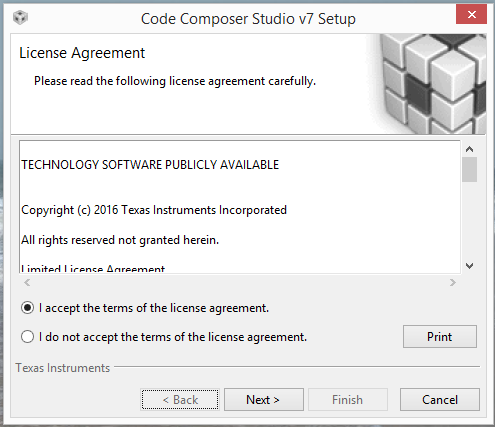
\includegraphics[width=6cm, height=6cm]{CCSInstall1}}
					\item Select the destination folder and click next.\\
							{\centering
							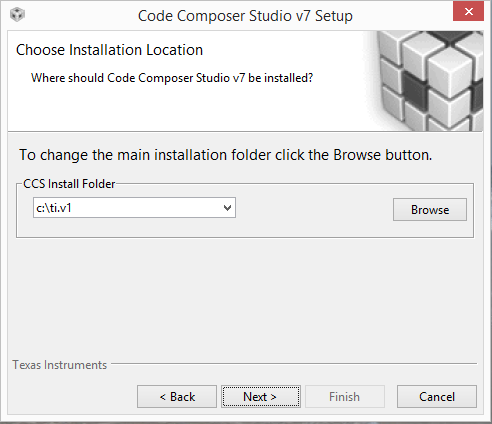
\includegraphics[width=6cm, height=6cm]{CCSInstall2}}
					\item Select the processors that your CCS installation will support. You
						must select "TM4C12X Arm Cortex M4". You can select other architectures, but the installation time and size will increase.\\{\centering
							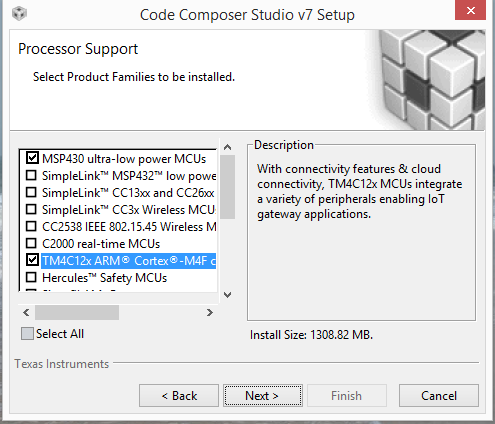
\includegraphics[width=6cm, height=6cm]{CCSInstall3}}
					\item Select debug probes and click finish \\
							{\centering
							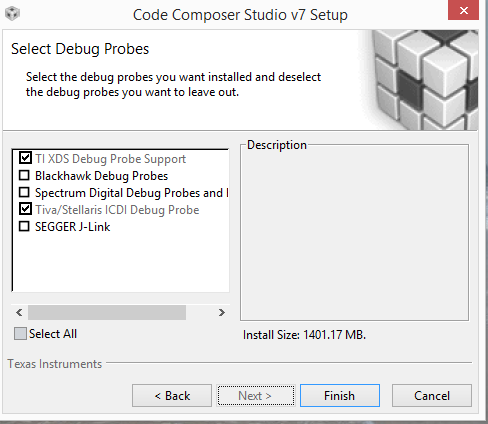
\includegraphics[width=6cm, height=6cm]{CCSInstall4}}
					\item The installer process	should take 15 - 30 minutes, depending on the speed of your connection. The offline
					installation should take 10 to 15 minutes. When the installation is complete, uncheck the
					“Launch Code Composer Studio v7” checkbox and then click Finish.There are several additional tools that require installation during the CCS install process. Click “Yes” or “OK” to proceed when these appear. \\
					\item Install TivaWare for C Series (Complete). Download and install the latest full version of TivaWare from: \href{http://www.ti.com/tool/sw-tm4c}{TivaWare}. The filename is SW-TM4C-x.x.exe . This
					workshop was built using version 1.1. Your version may be a later one. If at all possible,
					please install TivaWare into the default location.
				\end{enumerate}}
				{\large \textbf{\\You can find additional information at these websites:}\\
				Main page: www.ti.com/launchpad\\
				Tiva C Series TM4C123G LaunchPad:\\ http://www.ti.com/tool/ek-tm4c123gxl\\
				TM4C123GH6PM folder:\\ http://www.ti.com/product/tm4c123gh6pm\\
				BoosterPack webpage: www.ti.com/boosterpack\\
				LaunchPad Wiki:\\ www.ti.com/launchpadwiki\\}	\\	
				{\Large For understanding the launchpad properly and to learn more about Tiva it is strongly recommended to go through the webpage \href{http://processors.wiki.ti.com/index.php/Getting_Started_with_the_TIVA\%E2\%84\%A2_C_Series_TM4C123G_LaunchPad}{TIva Worshops} and download and read the workbook }
			\subsubsection{\Large \textbf{Create a New Project}}
				To create new project follow the steps mentioned:
				\begin{enumerate}
					\item Click File then New and then CCS Projects \\
						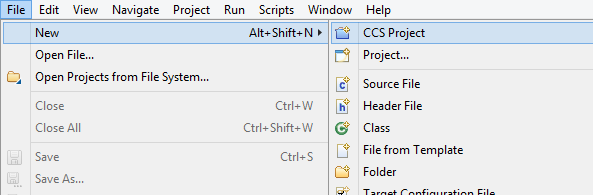
\includegraphics[width=6cm, height=2cm]{CreatingNewProject1}
					\item Select Target and connection as shown in the photo. Give a name to your project and save in a location.Click Finish. A main.c file will be open\\
						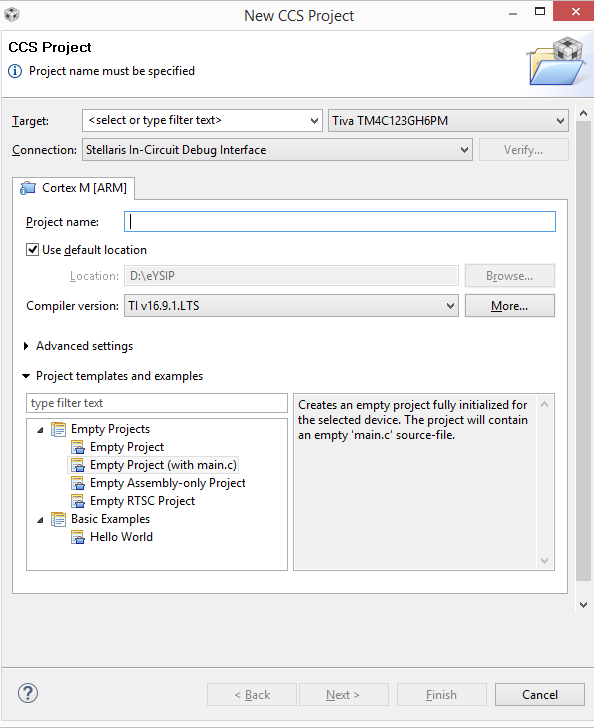
\includegraphics[width=6.5cm, height=8cm]{CreatingNewProject2}
				\end{enumerate}
			\subsubsection{\Large \textbf{Add Path and Build Variables}}
					{The path and build variables are used for:
					\begin{itemize}
						\item  Path variable – when you ADD (link) a file to your project, you can specify a "relative to" path. The default is PROJECT\_LOC which means that your linked resource (like a .lib	file) will be linked relative to your project directory.
						\item  Build variable – used for items such as the search path for include files associated with a library – i.e. it is used when you build your project.
				\end{itemize}
					Variables can either have a PROJECT scope (that they only work for this project) or a
					WORKSPACE scope (that they work across all projects in the workspace).
					In the next step, we need to add (link) a library file and then add a search path for include files.
					First, we’ll add these variables MANUALLY as WORKSPACE variables so that any project in your
					workspace can use the variables. Refer to the workbook by TI for adding as PROJECT}
				\paragraph{\Large \textbf{Adding a Path Variable}\\}
					To add a path variable,:
					\begin{itemize}
						\item Right-click on your Window Tab and select Preference.\\
							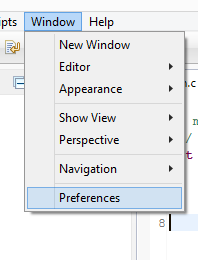
\includegraphics[width=3cm, height=4cm]{AddVariables}
						\item Expand General list  in the upper left-hand corner as shown and then expand the Resource list and click on Linked Resources:
						We want to add a New variable to specify exactly where you installed TivaWare.\\
						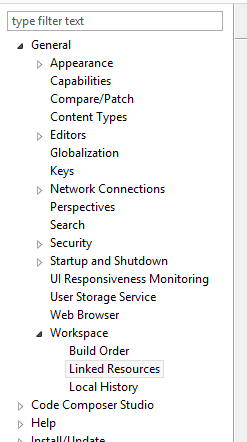
\includegraphics[height=8cm]{AddVariables2}
						\item Click New
						\item When the New Variable
						dialog appears,
						type TIVAWARE\_INSTALL
						for the name.\\
						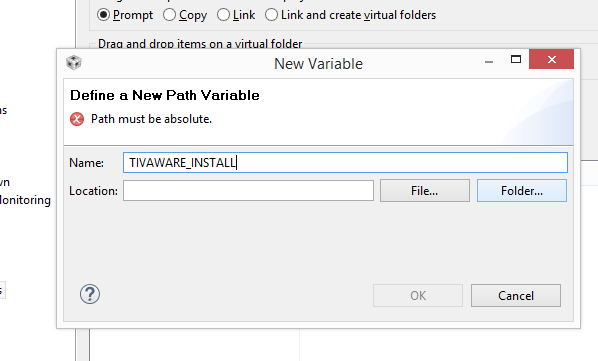
\includegraphics{AddVariables3}
						\item For the Location, click
						the Folder… button and
						navigate to your TivaWare
						installation. Click on the
						folder name and then click
						OK.\\
						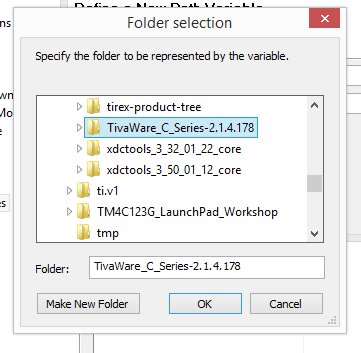
\includegraphics{AddVariables4}\\
						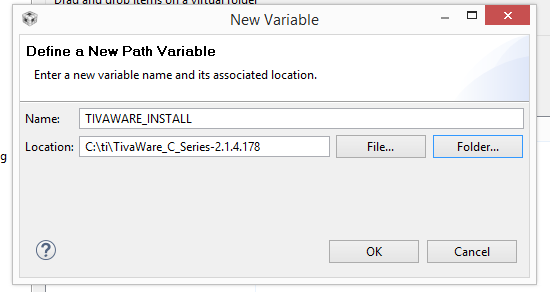
\includegraphics[width=9cm, height=8cm]{AddVariables5}
						\item Click OK. You should see your new variable listed in the Variables list.\\
						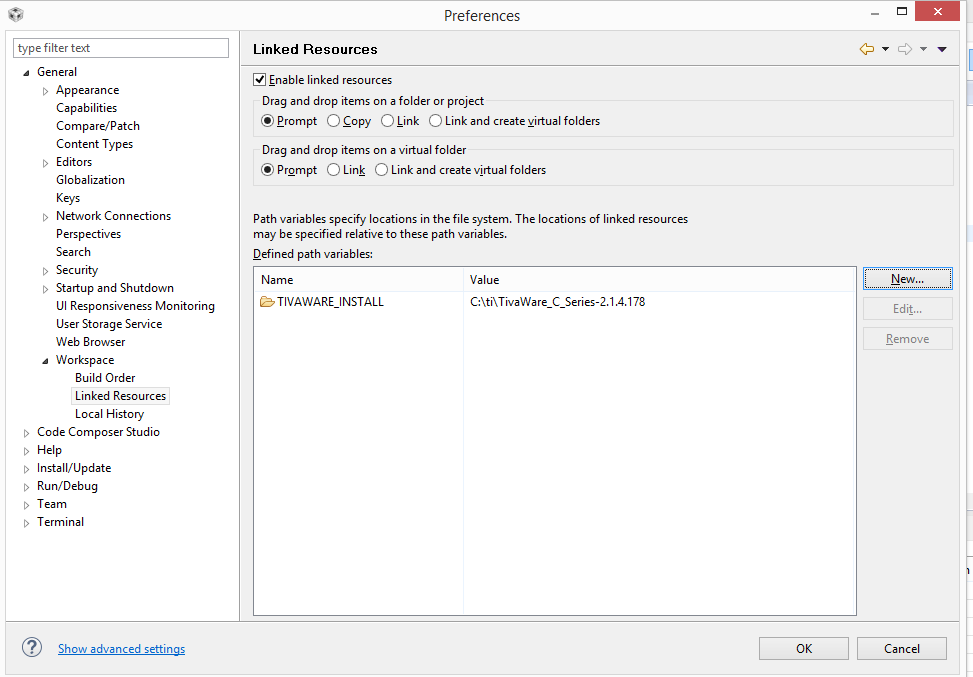
\includegraphics[width=10cm, height=8cm]{AddVariables6}
					\end{itemize}
					\paragraph{\Large \textbf{Adding a Build Variable}\\}
					Now let’s add a build variable that we will use in the include search path for the INCLUDE files
					associated with the TivaWare driver libraries.
					\begin{itemize}
						\item Click on Code Composer Studio Build and then the Variables tab:\\
							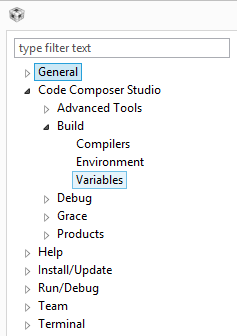
\includegraphics[width=7cm, height=8cm]{AddVariables7}\\
						\item Click the Add button. When the Define a New
						Build Variable dialog appears,
						insert TIVAWARE\_INSTALL into the Variables
						name box.\\
						\item Change the Type to Directory and
						browse to your Tivaware installation
						folder.\\
						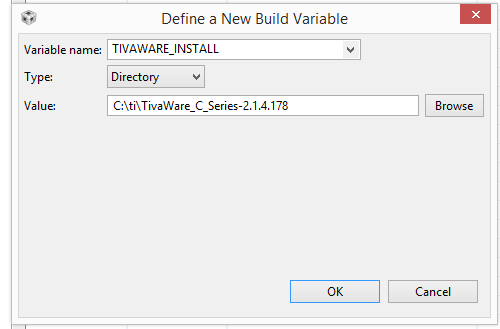
\includegraphics[width=10cm, height=8cm]{AddVariables8}
						\item  Click OK.
						\item  Click OK again to save and close
						the Build Properties window.\\
						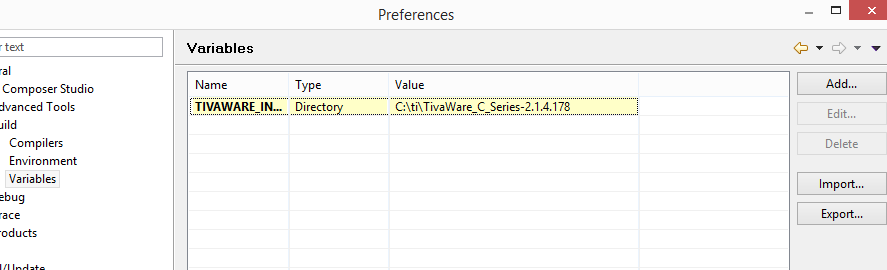
\includegraphics[width=20cm,height=10cm]{AddVariables9}
					\end{itemize}
		\subsection{\huge \textbf{driver.lib}}
		\subsection{\huge \textbf{Buzzer}}
		
			Located in the folder “Buzzer\_Beep” folder in the documentation.
			In this example, we will load buzzer beep code in Tiva based Fire Bird V. Now we will see in detail the structure of this code.This experiment demonstrates the simple operation of Buzzer ON/OFF with one second delay.
			Buzzer is connected to PORTF 4 pin of the Tiva Launchpad. If you have uC based board then it is connected to PORTA 2.
		
			\begin{lstlisting}[style=CStyle]
				#include <stdint.h>
				#include <stdbool.h>
				#include "inc/hw_types.h"
				#include "inc/hw_memmap.h"
				//This header File is important to Unlock GPIO Pins
				#include "inc/hw_gpio.h"
				#include "driverlib/sysctl.h"
				#include "driverlib/gpio.h"
				
				/**** Useful Macros Definition******/
				/******Remove the comments if you are using uC board******
				#define buzzerEnable    SYSCTL_PERIPH_GPIOA
				#define buzzer          GPIO_PORTA_BASE
				#define buzzerPin       GPIO_PIN_2
				**********************************************************/
				
				/******Remove the comments if you are using uC board******/
				#define buzzerEnable    SYSCTL_PERIPH_GPIOF
				#define buzzer          GPIO_PORTF_BASE
				#define buzzerPin       GPIO_PIN_4
				/**********************************************************/
				
				#define buzzerOn()      GPIOPinWrite(buzzer,buzzerPin,255)
				#define buzzerOff()     GPIOPinWrite(buzzer,buzzerPin,0)
				/***********************************/
				void setupCLK();
				void peripheralEnable();
				void configIOPin();
				void delay_ms(uint64_t delay);
				void delay_ms(uint64_t delay);
				
				int main(void) {
					setupCLK();
					peripheralEnable();
					configIOPin();
					while(1){
						buzzerOn();
						delay_ms(1000);
						buzzerOff();
						delay_ms(1000);
					}
				}
				/***************************************************************************************
				* This function is used to setup Clock frequency of the controller
				* It can be changed through codes
				* In this we have set frequency as 40Mhz
				* Frequency is set by SYSDIV which can be found in data sheet for different frequencies
				***************************************************************************************/
				void setupCLK(){
					SysCtlClockSet(SYSCTL_SYSDIV_5|SYSCTL_USE_PLL|SYSCTL_XTAL_16MHZ|SYSCTL_OSC_MAIN);
				}
				/*******************************
				* Enabling System Peripherals
				* buzzer Port in this case
				* buzzerPin for buzzer output
				******************************/
				void peripheralEnable(){
					SysCtlPeripheralEnable(buzzerEnable);
					/***** Just in case you are not familiar with macros*****
					SysCtlPeripheralEnable(SYSCTL_PERIPH_GPIOF);
					*************This is enabling PORTF*********************/
				}
				/*************************************
				* Configuring Pin as Input Or Output
				*************************************/
				void configIOPin(){
					GPIOPinTypeGPIOOutput(buzzer, buzzerPin);
					/***** Just in case you are not familiar with macros*****
					GPIOPinTypeGPIOOutput(buzzer, GPIO_PIN_4);
					*****************This is P4 output*********************/
				}
				/*********************************************
				* Calculating Delays
				* extern void SysCtlDelay(uint32_t ui32Count)
				* waits until the counting has been completed
				**********************************************/
				void delay_ms(uint64_t delay){
					SysCtlDelay(delay*SysCtlClockGet()/3000.0);
				}
				void delay_us(uint64_t delay){
					SysCtlDelay(delay*SysCtlClockGet()/3000000.0);
				}
			\end{lstlisting}
			
		\subsection{\huge \textbf{Programming the Robot}}
		\subsection{\huge \textbf{Using Debugger of The Programmer}}
		\subsection{\huge \textbf{Simple I/O Operation}}		
			{This experiment demonstrates the simple I/O operations.
			This example is only for plug and play board, but this should not discourage
			the user from understanding the example as it provide very important example of I/O operation 
			on TIVA platform.\\
			In this lab you have to use switch SW1, SW2 and RGB LED present on Tiva C series board.\\
			1. Use switch SW1 to Turn on Red LED on first switch press, Green LED on second
			switch press and Blue LED on third switch press. Repeat the same cycle next switch
			press onwards. Note that LED should remain on for the duration switch is kept pressed
			i.e. LED should turn off when switch is released.\\
			2. Use switch SW2 and sw2Status (a variable). Your program should increment sw2Status
			by one, every time switch is pressed. Note how the value of sw2Status changes on each
			switch press. Use debugger and add sw2Status to  Watch Expression" 	window.
			(You will find Continuous Refresh button on top of the Expression 	Window). You can
			use step debugging or breakpoints to check the variable value.
			Hint:To add variable to Expression Window, select and right click the variable name
			and select  Add Watch Expression". To view Expression Window, click on View button from CCS menu bar and select Expressions.}
			
			\begin{lstlisting}[style=CStyle]
				#include <stdint.h>
				#include <stdbool.h>
				#include "inc/hw_types.h"
				#include "inc/hw_memmap.h"
				#include "inc/hw_gpio.h" //To unlock locked pins for GPIO
				#include "driverlib/sysctl.h"
				#include "driverlib/gpio.h"
				#define userSwitch1 GPIO_PIN_0
				#define redLed      GPIO_PIN_1
				#define blueLed     GPIO_PIN_2
				#define greenLed    GPIO_PIN_3
				#define userSwitch2 GPIO_PIN_4
				#define LOCK_F (*((volatile unsigned long *)0x40025520))
				#define CR_F   (*((volatile unsigned long *)0x40025524))
				void setupCLK();
				void configIOPin();
				void delay_ms(uint64_t delay);
				void delay_us(uint64_t delay);
				
				int main(){
					setupCLK();
					SysCtlDelay(3);
					configIOPin();
					unsigned char pinData=1;
					unsigned char state=2;
					unsigned char countSwitch2=0;
					unsigned char flagSW1=0;
					unsigned char flagSW2=0;
					while(1){
						pinData=GPIOPinRead(GPIO_PORTF_BASE,userSwitch2|userSwitch1);
						if((pinData&0x01)==0)
							flagSW1=1;
						else if((flagSW1==1)&&(pinData&0x01)==1){
							countSwitch2+=1;
							flagSW1=0;
						}	
						if((pinData&0x10)==0){
							GPIOPinWrite(GPIO_PORTF_BASE,redLed|blueLed|greenLed,state);
							flagSW2=1;
						}
						else if(((flagSW2==1)&&(pinData&0x10)==0x10)){
							flagSW2=0;
							GPIOPinWrite(GPIO_PORTF_BASE,redLed|blueLed|greenLed,0);
							state=state*2;
							if(state>8)
								state=2;
						}
						delay_ms(5);
					}
				}
				/***************************************************************************************
				* This function is used to setup Clock frequency of the controller
				* Enabling System Peripherals
				* PORTF in this case
				******************************/
				void setupCLK(){
					SysCtlClockSet(SYSCTL_SYSDIV_4|SYSCTL_USE_PLL|SYSCTL_XTAL_16MHZ|SYSCTL_OSC_MAIN);
					SysCtlPeripheralEnable(SYSCTL_PERIPH_GPIOF);
				}
				/**********************************************
				* Configuring Pin as Input Or Output
				* PF0 by default is locked and cannot
				* be used as input unless it is unlocked
				***********************************************/
				void configIOPin(){
					GPIOPinTypeGPIOOutput(GPIO_PORTF_BASE, redLed|blueLed|greenLed);
					HWREG(GPIO_PORTF_BASE + GPIO_O_LOCK) = GPIO_LOCK_KEY;
					HWREG(GPIO_PORTF_BASE + GPIO_O_CR) |= 0x01;
					HWREG(GPIO_PORTF_BASE + GPIO_O_LOCK) = 0;
					GPIOPinTypeGPIOInput(GPIO_PORTF_BASE, userSwitch2|userSwitch1);
					GPIOPadConfigSet(GPIO_PORTF_BASE ,userSwitch2|userSwitch1,GPIO_STRENGTH_12MA,GPIO_PIN_TYPE_STD_WPU);
				}
				/*************************************
				* Calculating Delays
				*************************************/
				void delay_ms(uint64_t delay){
					SysCtlDelay(delay*(SysCtlClockGet()/3000));
				}
				void delay_us(uint64_t delay){
					SysCtlDelay(delay*(SysCtlClockGet()/3000000UL));
				}
			\end{lstlisting}
		
		\subsection{\huge \textbf{Robot Direction Control}}
			{Located in the folder “Experiments \ Motion Control Simple” folder. Robot’s motors are controlled by L293D motor controller. Using L293D, microcontroller can control direction and velocity of both of the motors. To change the direction appropriate logic levels (High/Low) are applied to IC L293D’s direction pins. Velocity control is done using pulse width modulation (PWM) applied to Enable pins of L293D IC.\\}
			
			The Motor connections are as shown below 
			
			\begin{center}
				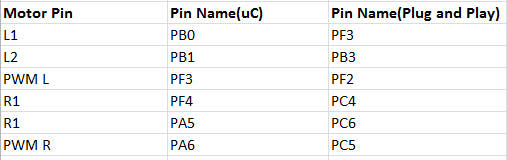
\includegraphics[width=6cm, height=2cm]{MotorConnection}
			\end{center}
			
			\textbf{Code for Plug and Play Board:}
			\begin{lstlisting}[style=CStyle]
				#include <stdint.h>
				#include <stdbool.h>
				#include "inc/hw_types.h"
				#include "inc/hw_memmap.h"
				//This header File is important to Unlock GPIO Pins
				#include "inc/hw_gpio.h"
				#include "driverlib/sysctl.h"
				#include "driverlib/gpio.h"
				//Used for controlling Motor direction
				#define right           0x41
				#define left            0x18
				#define softRight       0x10
				#define softLeft        0x01
				#define forward         0x11
				#define backward        0x48
				
				void setupCLK();
				void peripheralEnable();
				void configIOPin();
				void delay_ms(uint64_t delay);
				void delay_us(uint64_t delay);
				void motion(uint8_t);
				
				int main(void) {
					setupCLK();
					peripheralEnable();
					configIOPin();
					while(1){
						motion(forward);
						delay_ms(1000);
						motion(right);
						delay_ms(1000);
						motion(left);
						delay_ms(1000);
						motion(backward);
						delay_ms(1000);
					}
				}
				/***************************************************************************************
				* This function is used to setup Clock frequency of the controller
				* It can be changed through codes
				* In this we have set frequency as 40Mhz
				* Frequency is set by SYSDIV which can be found in data sheet for different frequencies
				***************************************************************************************/
				void setupCLK(){
					SysCtlClockSet(SYSCTL_SYSDIV_5|SYSCTL_USE_PLL|SYSCTL_XTAL_16MHZ|SYSCTL_OSC_MAIN);
				}
				/*******************************
				* Enabling System Peripherals
				* PORTF,PORTB and PORTC in this case
				******************************/
				void peripheralEnable(){
					SysCtlPeripheralEnable(SYSCTL_PERIPH_GPIOB);
					SysCtlPeripheralEnable(SYSCTL_PERIPH_GPIOF);
					SysCtlPeripheralEnable(SYSCTL_PERIPH_GPIOC);
				}
				/*************************************
				* Configuring Pin as Input Or Output
				* And Setting PWM Pin to Always High
				*************************************/
				void configIOPin(){
					GPIOPinTypeGPIOOutput(GPIO_PORTB_BASE,GPIO_PIN_3);
					GPIOPinTypeGPIOOutput(GPIO_PORTC_BASE,GPIO_PIN_4|GPIO_PIN_5|GPIO_PIN_6);
					GPIOPinTypeGPIOOutput(GPIO_PORTF_BASE,GPIO_PIN_3|GPIO_PIN_2);
					GPIOPinWrite(GPIO_PORTF_BASE,GPIO_PIN_2,255);
					GPIOPinWrite(GPIO_PORTC_BASE,GPIO_PIN_5,255);
				}
				/*************************************
				* Calculating Delays
				*************************************/
				void delay_ms(uint64_t delay){
					SysCtlDelay(delay*(SysCtlClockGet()/3000));
				}
				void delay_us(uint64_t delay){
					SysCtlDelay(delay*(SysCtlClockGet()/3000000UL));
				}
				/******************************************************
				* This function is for giving the direction of motion
				* Macros have been defined at starting
				* Macros for directions are 8 bits
				* Out of these 8 bits only 4 are used
				* Bit 0 (LSB) corresponds to PB3
				* Bit 3       corresponds to PF3
				* Bit 4       corresponds to PC4
				* Bit 6       corresponds to PF6
				*****************************************************/
				void motion(uint8_t direction){
					GPIOPinWrite(GPIO_PORTB_BASE,GPIO_PIN_3,direction<<3);
					GPIOPinWrite(GPIO_PORTC_BASE,GPIO_PIN_4|GPIO_PIN_6,direction);
					GPIOPinWrite(GPIO_PORTF_BASE,GPIO_PIN_3,direction);
				}
			\end{lstlisting}
	
			\textbf{Code for uC based Board:}
			\begin{lstlisting}[style=CStyle]
				#include <stdint.h>
				#include <stdbool.h>
				#include "inc/hw_types.h"
				#include "inc/hw_memmap.h"
				//This header File is important to Unlock GPIO Pins
				#include "inc/hw_gpio.h"
				#include "driverlib/sysctl.h"
				#include "driverlib/gpio.h"	
				//Used for control Motor direction
				#define right           0x22
				#define left            0x11
				#define softRight       0x02
				#define softLeft        0x10
				#define forward         0x12
				#define backward        0x21
				#define stop            0x00
			
				void setupCLK();
				void peripheralEnable();
				void configIOPin();
				void delay_ms(uint64_t delay);
				void delay_ms(uint64_t delay);
				void motion(uint8_t);
				
				int main(void) {
					setupCLK();
					peripheralEnable();
					configIOPin();
					while(1){
						motion(forward);
						delay_ms(1000);
						motion(right);
						delay_ms(1000);
						motion(left);
						delay_ms(1000);
						motion(backward);
						delay_ms(1000);
					}
				}
				/***************************************************************************************
				* This function is used to setup Clock frequency of the controller
				* It can be changed through codes
				* In this we have set frequency as 40Mhz
				* Frequency is set by SYSDIV which can be found in data sheet for different frequencies
				***************************************************************************************/
				void setupCLK(){
					SysCtlClockSet(SYSCTL_SYSDIV_5|SYSCTL_USE_PLL|SYSCTL_XTAL_16MHZ|SYSCTL_OSC_MAIN);
				}
				/*******************************
				* Enabling System Peripherals
				* PORTF,PORTB and PORTC in this case
				******************************/
				void peripheralEnable(){
					SysCtlPeripheralEnable(SYSCTL_PERIPH_GPIOB);
					SysCtlPeripheralEnable(SYSCTL_PERIPH_GPIOF);
					SysCtlPeripheralEnable(SYSCTL_PERIPH_GPIOA);
				}
				/*************************************
				* Configuring Pin as Input Or Output
				* And Setting PWM Pin to Always High
				*************************************/
				void configIOPin(){
					GPIOPinTypeGPIOOutput(GPIO_PORTB_BASE,GPIO_PIN_0|GPIO_PIN_1);
					GPIOPinTypeGPIOOutput(GPIO_PORTA_BASE,GPIO_PIN_6|GPIO_PIN_5);
					GPIOPinTypeGPIOOutput(GPIO_PORTF_BASE,GPIO_PIN_4|GPIO_PIN_3);
					GPIOPinWrite(GPIO_PORTF_BASE,GPIO_PIN_3,255);
					GPIOPinWrite(GPIO_PORTA_BASE,GPIO_PIN_6,255);
				}
				/*************************************
				* Calculating Delays
				*************************************/
				void delay_ms(uint64_t delay){
					SysCtlDelay(delay*(SysCtlClockGet()/3000));
				}
				void delay_us(uint64_t delay){
					SysCtlDelay(delay*(SysCtlClockGet()/3000000UL));
				}
				/******************************************************
				* This function is for giving the direction of motion
				* Macros have been defined at starting
				* Macros for directions are 8 bits
				* Out of these 8 bits only 4 are used
				* Bit 0 (LSB) corresponds to PB0
				* Bit 1       corresponds to PF1
				* Bit 4       corresponds to PF4
				* Bit 5       corresponds to PA5
				*****************************************************/
				void motion(uint8_t direction){
					GPIOPinWrite(GPIO_PORTB_BASE,GPIO_PIN_0|GPIO_PIN_1,direction);
					GPIOPinWrite(GPIO_PORTA_BASE,GPIO_PIN_5,direction);
					GPIOPinWrite(GPIO_PORTF_BASE,GPIO_PIN_4,direction);
				}
			\end{lstlisting}
		\subsection{\huge \textbf{Robot Position Control Using Interrupts}}
			{Position encoders give position / velocity feedback to the robot. It is used in closed loop to control robot’s position and velocity.  Position encoder consists of optical  encoder and slotted disc assembly. When this slotted disc moves in between the optical encoder we get square wave signal whose pulse  count  indicates  position  and  time  period indicates  velocity.}\\
			
			\textbf{Connections:\\}
			\begin{center}
				
				\textbf{Plug and Play Board:}\\
				PB2 : External interrupt for left motor position encoder\\
				PF0 : External interrupt for the right position encoder\\
			
				\textbf{uC Based Board:}\\
				PA4 : External interrupt for left motor position encoder\\
				PA3 : External interrupt for the right position encoder\\
			\end{center}
			\subsubsection{\textbf{Calculation of position encoder resolution:}}	
			To be added later
			
			\textbf{Code for Plug and Play Board:}
			\begin{lstlisting}[style=CStyle]
				#include <stdint.h>
				#include <stdbool.h>
				#include "inc/tm4c123gh6pm.h"
				#include "inc/hw_memmap.h"
				#include "inc/hw_types.h"
				#include "inc/hw_gpio.h"
				#include "driverlib/sysctl.h"
				#include "driverlib/interrupt.h"
				#include "driverlib/gpio.h"
				//This header File is important to Unlock GPIO Pins
				#include "inc/hw_gpio.h"
				#include "driverlib/sysctl.h"
				#include "driverlib/gpio.h"
				
				#define right           0x41
				#define left            0x18
				#define softRight       0x10
				#define softLeft        0x01
				#define forward         0x11
				#define backward        0x48
				#define stop            0x00
				
				void setupCLK();
				void peripheralEnable();
				void configIOPin();
				void delay_ms(uint64_t delay);
				void delay_us(uint64_t delay);
				void motion(uint8_t);
				void interruptEnable();
				void encoderInterruptEncountered();
				void encoderInterruptEncountered1();
				void angleRotate(uint16_t Degrees);
				void linearDistanceMM(unsigned int DistanceInMM);
				void rightDegrees(unsigned int Degrees);
				void leftDegrees(unsigned int Degrees);
				void forwardMM(unsigned int DistanceInMM);
				void backwardMM(unsigned int DistanceInMM);
				volatile unsigned long int ShaftCountRight = 0;
				volatile unsigned long int ShaftCountLeft = 0;
				
				int main(void) {
					setupCLK();
					peripheralEnable();
					configIOPin();
					interruptEnable();
					while(1){
						forwardMM(100);
						delay_ms(1000);
						leftDegrees(90);
						delay_ms(1000);
					}
				}
				/***************************************************************************************
				* This function is used to setup Clock frequency of the controller
				* It can be changed through codes
				* In this we have set frequency as 40Mhz
				* Frequency is set by SYSDIV which can be found in data sheet for different frequencies
				***************************************************************************************/
				void setupCLK(){
					SysCtlClockSet(SYSCTL_SYSDIV_5|SYSCTL_USE_PLL|SYSCTL_XTAL_16MHZ|SYSCTL_OSC_MAIN);
				}
				/*******************************
				* Enabling System Peripherals
				* PORTF,PORTB and PORTC in this case
				******************************/
				void peripheralEnable(){
					SysCtlPeripheralEnable(SYSCTL_PERIPH_GPIOB);
					SysCtlPeripheralEnable(SYSCTL_PERIPH_GPIOF);
					SysCtlPeripheralEnable(SYSCTL_PERIPH_GPIOC);
				}
				/*************************************
				* Configuring Pin as Input Or Output
				* Unlocking PF0
				* Setting PWM Pins to Always High
				* Weak Pull to the Input Pins
				*************************************/
				void configIOPin(){
					GPIOPinTypeGPIOOutput(GPIO_PORTB_BASE,GPIO_PIN_3);
					GPIOPinTypeGPIOOutput(GPIO_PORTC_BASE,GPIO_PIN_4|GPIO_PIN_5|GPIO_PIN_6);
					GPIOPinTypeGPIOOutput(GPIO_PORTF_BASE,GPIO_PIN_3|GPIO_PIN_2|GPIO_PIN_1);
					GPIOPinWrite(GPIO_PORTF_BASE,GPIO_PIN_2,255);
					GPIOPinWrite(GPIO_PORTC_BASE,GPIO_PIN_5,255);
					HWREG(GPIO_PORTF_BASE + GPIO_O_LOCK) = GPIO_LOCK_KEY;
					HWREG(GPIO_PORTF_BASE + GPIO_O_CR) |= 0x01;
					HWREG(GPIO_PORTF_BASE + GPIO_O_LOCK) = 0;
					GPIOPinTypeGPIOInput(GPIO_PORTF_BASE, GPIO_PIN_0);
					GPIOPadConfigSet(GPIO_PORTF_BASE,GPIO_PIN_0,GPIO_STRENGTH_2MA,GPIO_PIN_TYPE_STD_WPU);
					GPIOPinTypeGPIOInput(GPIO_PORTB_BASE, GPIO_PIN_2);
					GPIOPadConfigSet(GPIO_PORTB_BASE,GPIO_PIN_2,GPIO_STRENGTH_2MA,GPIO_PIN_TYPE_STD_WPU);
				}
				/*************************************
				* Calculating Delays
				*************************************/
				void delay_ms(uint64_t delay){
					SysCtlDelay(delay*(SysCtlClockGet()/3000));
				}
				void delay_us(uint64_t delay){
					SysCtlDelay(delay*(SysCtlClockGet()/3000000UL));
				}
				/******************************************************
				* This function is for giving the direction of motion
				* Macros have been defined at starting
				* Macros for directions are 8 bits
				* Out of these 8 bits only 4 are used
				* Bit 0 (LSB) corresponds to PB3
				* Bit 3       corresponds to PF3
				* Bit 4       corresponds to PC4
				* Bit 6       corresponds to PF6
				*****************************************************/
				void motion(uint8_t direction){
					GPIOPinWrite(GPIO_PORTB_BASE,GPIO_PIN_3,direction<<3);
					GPIOPinWrite(GPIO_PORTC_BASE,GPIO_PIN_4|GPIO_PIN_6,direction);
					GPIOPinWrite(GPIO_PORTF_BASE,GPIO_PIN_3,direction);
					}
					/****For Enabling Interrupt on PORTF and PORTB****/
					void interruptEnable(){
					GPIOIntDisable(GPIO_PORTF_BASE,GPIO_PIN_0);
					GPIOIntClear(GPIO_PORTF_BASE,GPIO_PIN_0);
					GPIOIntRegister(GPIO_PORTF_BASE, encoderInterruptEncountered);
					GPIOIntTypeSet(GPIO_PORTF_BASE,GPIO_PIN_0,GPIO_FALLING_EDGE);
					GPIOIntEnable(GPIO_PORTF_BASE,GPIO_PIN_0);			
					GPIOIntDisable(GPIO_PORTB_BASE,GPIO_PIN_2);
					GPIOIntClear(GPIO_PORTB_BASE,GPIO_PIN_2);
					GPIOIntRegister(GPIO_PORTB_BASE, encoderInterruptEncountered1);
					GPIOIntTypeSet(GPIO_PORTB_BASE,GPIO_PIN_2,GPIO_FALLING_EDGE);
					GPIOIntEnable(GPIO_PORTB_BASE,GPIO_PIN_2);
				}	
				/**** ISR For External Interrupt on PortF************************
				* Check on which pin of the PORTA has encountered an interrupt
				* There is only one ISR for complete PORT
				* No two PORTs can have same ISR
				****************************************************************/
				void encoderInterruptEncountered(){
					if(GPIOIntStatus(GPIO_PORTF_BASE, false)&GPIO_PIN_0){
						ShaftCountRight++;
						GPIOIntClear(GPIO_PORTF_BASE, GPIO_PIN_0);
					}
					if(GPIOIntStatus(GPIO_PORTB_BASE, false)&GPIO_PIN_2){
						ShaftCountLeft++;
						GPIOPinWrite(GPIO_PORTF_BASE,GPIO_PIN_1,2);
						GPIOIntClear(GPIO_PORTB_BASE, GPIO_PIN_2);
					}
				}
				/****************************************************
				* Function to Rotate to desired Angle
				* Resolution can be Change to Get Higher Precision
				****************************************************/
				void angleRotate(uint16_t Degrees){
					unsigned long int ReqdShaftCountInt = 0;
					ReqdShaftCountInt = Degrees/ 4.09;// division by resolution to get shaft count
					ShaftCountRight = 0;
					while (1){
						if((ShaftCountRight>=ReqdShaftCountInt))
							break;
					}
					motion(stop);
				}
				/****************************************************
				* Function to Move in a Linear Distance
				* Resolution can be Change to Get Higher Precision
				****************************************************/
				void linearDistanceMM(unsigned int DistanceInMM){
					unsigned long int ReqdShaftCountInt = 0;
					ReqdShaftCountInt =DistanceInMM / 5.338;;
					ShaftCountRight=0;
					ShaftCountLeft=0;
					while(1){
						if((ShaftCountRight >=ReqdShaftCountInt)&&(ShaftCountLeft >= ReqdShaftCountInt))
							break;
						else if((ShaftCountRight > ReqdShaftCountInt))
							motion(softRight);
						else if((ShaftCountLeft > ReqdShaftCountInt))
							motion(softLeft);
					}
					motion(stop); //Stop robot
				}
				void forwardMM(unsigned int DistanceInMM){
					motion(forward);
					linearDistanceMM(DistanceInMM);
				}
				
				void backwardMM(unsigned int DistanceInMM){
					motion(backward);
					linearDistanceMM(DistanceInMM);
				}
				void leftDegrees(unsigned int Degrees){
					motion(left); //Turn left
					angleRotate(Degrees);
				}
				void rightDegrees(unsigned int Degrees){
					motion(right); //Turn right
					angleRotate(Degrees);
				}
			\end{lstlisting}	
			
			\textbf{Code for uC based Board:}
			\begin{lstlisting}[style=CStyle]
				#include <stdint.h>
				#include <stdbool.h>
				#include "inc/tm4c123gh6pm.h"
				#include "inc/hw_memmap.h"
				#include "inc/hw_types.h"
				#include "inc/hw_gpio.h"
				#include "driverlib/sysctl.h"
				#include "driverlib/interrupt.h"
				#include "driverlib/gpio.h"
				
				#define right           0x22
				#define left            0x11
				#define softRight       0x02
				#define softLeft        0x10
				#define forward         0x12
				#define backward        0x21
				#define stop            0x00
				
				void setupCLK();
				void peripheralEnable();
				void gpioEnable();
				void interruptEnable();
				void encoderInterruptEncountered();
				void linearDistanceMM(unsigned int);
				void angleRotate(uint16_t);
				void forwardMM(unsigned int);
				void backwardMM(unsigned int);
				void leftDegrees(unsigned int);
				void rightDegrees(unsigned int);
				void delay_ms(uint64_t delay);
				void delay_us(uint64_t delay);
				void motion(uint8_t direction);
				volatile uint16_t ShaftCountRight=0,ShaftCountLeft=0;
				
				int main(void) {
					setupCLK();
					peripheralEnable();
					gpioEnable();
					interruptEnable();
					while(1){
						forwardMM(100);
						delay_ms(1000);
						rightDegrees(90);
						delay_ms(1000);
					}
				}
				
				/***************************************************************************************
				* This function is used to setup Clock frequency of the controller
				* It can be changed through codes
				* In this we have set frequency as 40Mhz
				* Frequency is set by SYSDIV which can be found in data sheet for different frequencies
				***************************************************************************************/
				void setupCLK(){
					SysCtlClockSet(SYSCTL_SYSDIV_5|SYSCTL_USE_PLL|SYSCTL_XTAL_16MHZ|SYSCTL_OSC_MAIN);
				}
				
				/*******************************
				* Enabling System Peripherals
				* PORTF,PORTB and PORTA in this case
				******************************/
				void peripheralEnable(){
					SysCtlPeripheralEnable(SYSCTL_PERIPH_GPIOB);
					SysCtlPeripheralEnable(SYSCTL_PERIPH_GPIOF);
					SysCtlPeripheralEnable(SYSCTL_PERIPH_GPIOA);
				}
				
				/*************************************
				* Configuring Pin as Input Or Output
				* Setting PWM Pins to Always High
				* Weak Pull to the Input Pins
				*************************************/
				void gpioEnable(){
					GPIOPinTypeGPIOOutput(GPIO_PORTF_BASE,GPIO_PIN_1|GPIO_PIN_2);
					GPIOPinTypeGPIOOutput(GPIO_PORTB_BASE,GPIO_PIN_0|GPIO_PIN_1);
					GPIOPinTypeGPIOOutput(GPIO_PORTA_BASE,GPIO_PIN_6|GPIO_PIN_5);
					GPIOPinTypeGPIOOutput(GPIO_PORTF_BASE,GPIO_PIN_4|GPIO_PIN_3);
					GPIOPinWrite(GPIO_PORTF_BASE,GPIO_PIN_3,255);
					GPIOPinWrite(GPIO_PORTA_BASE,GPIO_PIN_6,255);
					GPIOPinTypeGPIOInput(GPIO_PORTA_BASE, GPIO_PIN_4|GPIO_PIN_3);
					GPIOPadConfigSet(GPIO_PORTA_BASE ,GPIO_PIN_4|GPIO_PIN_5,GPIO_STRENGTH_2MA,GPIO_PIN_TYPE_STD_WPU);
				}
				/****For Enabling Interrupt on PortA****/
				void interruptEnable(){
					GPIOIntDisable(GPIO_PORTA_BASE,GPIO_PIN_4|GPIO_PIN_3);
					GPIOIntClear(GPIO_PORTA_BASE, GPIO_PIN_4|GPIO_PIN_3);
					GPIOIntRegister(GPIO_PORTA_BASE, encoderInterruptEncountered);
					GPIOIntTypeSet(GPIO_PORTA_BASE,GPIO_PIN_4|GPIO_PIN_3,GPIO_FALLING_EDGE);
					GPIOIntEnable(GPIO_PORTA_BASE,GPIO_PIN_4|GPIO_PIN_3);
				}
				/**** ISR For External Interrupt on PortA************************
				* Check on which pin of the PORTA has encountered an interrupt
				* There is only one ISR for complete PORT
				* No two PORTs can have same ISR
				****************************************************************/
				void encoderInterruptEncountered(){
					if(GPIOIntStatus(GPIO_PORTA_BASE, false)&GPIO_PIN_4){
						ShaftCountLeft++;
						GPIOIntClear(GPIO_PORTA_BASE, GPIO_PIN_4);
					}
					if(GPIOIntStatus(GPIO_PORTA_BASE, false)&GPIO_PIN_3){
						ShaftCountRight++;
						GPIOIntClear(GPIO_PORTA_BASE, GPIO_PIN_3);
					}
				}
				/*************************************
				* Calculating Delays
				*************************************/
				void delay_ms(uint64_t delay){
					SysCtlDelay(delay*(SysCtlClockGet()/3000));
				}
				void delay_us(uint64_t delay){
					SysCtlDelay(delay*(SysCtlClockGet()/3000000UL));
				}
				/******************************************************
				* This function is for giving the direction of motion
				* Macros have been defined at starting
				* Macros for directions are 8 bits
				* Out of these 8 bits only 4 are used
				* Bit 0 (LSB) corresponds to PB3
				* Bit 3       corresponds to PF3
				* Bit 4       corresponds to PC4
				* Bit 6       corresponds to PF6
				*****************************************************/
				void motion(uint8_t direction){
					GPIOPinWrite(GPIO_PORTB_BASE,GPIO_PIN_0|GPIO_PIN_1,direction);
					GPIOPinWrite(GPIO_PORTA_BASE,GPIO_PIN_5,direction);
					GPIOPinWrite(GPIO_PORTF_BASE,GPIO_PIN_4,direction);
				}
				/****************************************************
				* Function to Rotate to desired Angle
				* Resolution can be Change to Get Higher Precision
				****************************************************/
				void angleRotate(uint16_t Degrees){
					unsigned long int ReqdShaftCountInt = 0;  // division by resolution to get shaft count
					ReqdShaftCountInt = Degrees/ 4.09;;
					ShaftCountRight = 0;
					ShaftCountLeft = 0;
					while (1){
						if((ShaftCountRight>=ReqdShaftCountInt)&&(ShaftCountLeft>=ReqdShaftCountInt))
							break;
					}
					motion(stop);
				}
				/****************************************************
				* Function to Move in a Linear Distance
				* Resolution can be Change to Get Higher Precision
				****************************************************/
				void linearDistanceMM(unsigned int DistanceInMM){
					unsigned long int ReqdShaftCountInt = 0;
					ReqdShaftCountInt =DistanceInMM / 5.338;;
					ShaftCountRight=0;
					ShaftCountLeft=0;
					while(1){
						if((ShaftCountRight > ReqdShaftCountInt)&&(ShaftCountLeft > ReqdShaftCountInt))
							break;
						else if((ShaftCountRight > ReqdShaftCountInt))
							motion(softRight);
						else if((ShaftCountLeft > ReqdShaftCountInt))
						motion(softLeft);
					}
					motion(stop); //Stop robot
				}
				void forwardMM(unsigned int DistanceInMM){
					motion(forward);
					linearDistanceMM(DistanceInMM);
				}	
				void backwardMM(unsigned int DistanceInMM){
					motion(backward);
					linearDistanceMM(DistanceInMM);
				}
				void leftDegrees(unsigned int Degrees){
					motion(left); //Turn left
					angleRotate(Degrees);
				}
				void rightDegrees(unsigned int Degrees){
					motion(right); //Turn right
					angleRotate(Degrees);
				}
			\end{lstlisting}
			
		\subsection{\huge \textbf{Timers and its Interrupts}}
			{The TM4C123GH6PM General-Purpose Timer Module (GPTM) contains six 16/32-bit GPTM blocks	and six 32/64-bit Wide GPTM blocks. Each 16/32-bit GPTM block provides two 16-bit timers/counters	(referred to as Timer A and Timer B) that can be configured to operate independently as timers or event counters, or concatenated to operate as one 32-bit timer or one 32-bit Real-Time Clock (RTC). Each 32/64-bit Wide GPTM block provides 32-bit timers for Timer A and Timer B that can be concatenated to operate as a 64-bit timer.}\\
			
			Timers are mainly used for
			\begin{itemize}
				\item Velocity Control
				\item Servo Motor Control
				\item Event Scheduling
				\item Velocity Calculation
			\end{itemize}
			
			In this section the event scheduling application of timer is explained. To illustrate this the buzzer is switched On and OFF periodically. The remaining applications are explained in the further sections. \\
			
			\begin{lstlisting}[style=CStyle]
				#include <stdint.h>
				#include <stdbool.h>
				#include "inc/hw_types.h"
				#include "inc/hw_memmap.h"
				#include "inc/tm4c123gh6pm.h"
				//This header File is important to Unlock GPIO Pins
				#include "inc/hw_gpio.h"
				#include "driverlib/sysctl.h"
				#include "driverlib/gpio.h"
				//Used for enabling the timer
				#include "driverlib/timer.h"
				//Used for enabling interrupt
				#include "driverlib/interrupt.h"
				/**** Useful Macros Definition******/
				/******Remove the comments if you are using uC board******
				#define buzzerEnable    SYSCTL_PERIPH_GPIOA
				#define buzzer          GPIO_PORTA_BASE
				#define buzzerPin       GPIO_PIN_2
				**********************************************************/
				
				/******Remove the comments if you are using uC board******/
				#define buzzerEnable    SYSCTL_PERIPH_GPIOF
				#define buzzer          GPIO_PORTF_BASE
				#define buzzerPin       GPIO_PIN_4
				/**********************************************************/
				
				#define buzzerOn()      GPIOPinWrite(buzzer,buzzerPin,255)
				#define buzzerOff()     GPIOPinWrite(buzzer,buzzerPin,0)
				/***********************************/
				void setupCLK();
				void peripheralEnable();
				void configIOPin();
				void timerEnable();
				
				uint32_t ui32Period;    // used for generating one second delay
				volatile int flag = 0;           //used to monitor the state of buzzer
				
				int main(void) {
					setupCLK();
					peripheralEnable();
					configIOPin();
					timerEnable();
					flag = 0;
					while(1){
					}
				}
				/***************************************************************************************
				* This function is used to setup Clock frequency of the controller
				* It can be changed through codes
				* In this we have set frequency as 40Mhz
				* Frequency is set by SYSDIV which can be found in data sheet for different frequencies
				***************************************************************************************/
				void setupCLK(){
					SysCtlClockSet(SYSCTL_SYSDIV_5|SYSCTL_USE_PLL|SYSCTL_XTAL_16MHZ|SYSCTL_OSC_MAIN);
				}
				/*******************************
				* Enabling System Peripherals
				* buzzer Port in this case
				* buzzerPin for buzzer output
				* Enabling Timer 0
				******************************/
				void peripheralEnable(){
					SysCtlPeripheralEnable(buzzerEnable);
					SysCtlPeripheralEnable(SYSCTL_PERIPH_TIMER0);
					/***** Just in case you are not familiar with macros*****
					SysCtlPeripheralEnable(SYSCTL_PERIPH_GPIOF);
					*************This is enabling PORTF*********************/
				}
				/*************************************
				* Configuring Pin as Input Or Output
				*************************************/
				void configIOPin(){
					GPIOPinTypeGPIOOutput(buzzer, buzzerPin);
				}
				/*******************************
				* Enabling Timer 0
				* Timer is configured to be generate
				interrupt every second
				* Here sysCtlClockGet() is divided
				by the on time of buzzer
				******************************/
				void timerEnable(){
					TimerConfigure(TIMER0_BASE, TIMER_CFG_PERIODIC);
					ui32Period = (SysCtlClockGet() / 1) / 2;
					TimerLoadSet(TIMER0_BASE, TIMER_A, ui32Period -1);
					IntEnable(INT_TIMER0A);
					TimerIntEnable(TIMER0_BASE, TIMER_TIMA_TIMEOUT);
					IntMasterEnable();
					TimerEnable(TIMER0_BASE, TIMER_A);
				}
				/*******************************************************************
				* This function is executed when the timer overflows
				* In this example the buzzer is switched on and off alternatively
				*******************************************************************/
				void Timer0IntHandler(void)
				{
				// Clear the timer interrupt
					TimerIntClear(TIMER0_BASE, TIMER_TIMA_TIMEOUT);
					flag = !flag;
					if(flag == 0){
						buzzerOn();
					}
					else{
						buzzerOff();
					}
				}
			\end{lstlisting}
			 
		\subsection{\huge \textbf{Robot Speed Control}}
			\subsubsection{\textbf{Pulse Width Modulation(PWM)}}
				Pulse width modulation is a process in which duty cycle of constant frequency square wave is modulated to control power delivered to the load i.e. motor. \\
				Duty cycle is the ratio of ‘T-ON/ T’. Where ‘T-ON’ is ON time and ‘T’ is the time period of the wave. Power delivered to the motor is proportional to the ‘T-ON’ time of the signal. In case of PWM the motor reacts to the time average of the signal. \\
				PWM is used to control total amount of power delivered to the load without power losses which generally occur in resistive methods of power control. 
				\begin{center}
					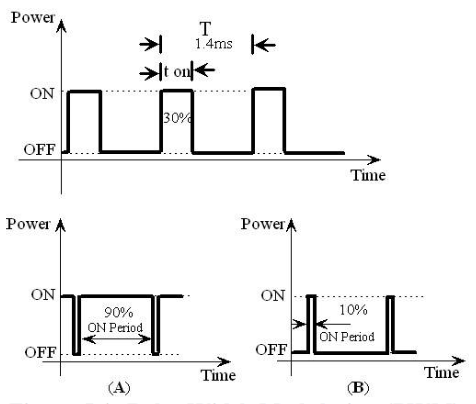
\includegraphics[width=4cm, height=4cm]{PWM}
				\end{center}
				Above figure shows the PWM waveforms for motor velocity control. In case (A), ON time is
				90 percent of time period. This wave has more average value. Hence more power is delivered to themotor. In case (B), the motor will run slower as the ON time is just 10 percent of time period. \\
				
				\hspace{-.7cm}
				The TM4C123GH6PM microcontroller contains two PWM modules, each with four PWM generator blocks and a control block, for a total of 16 PWM outputs. The control block determines the polarity of the PWM signals, and which signals are passed through to the pins. The connections of PWM motor pins are given in the section 6.7. The same code is modified to change the velocity of the motors.
				
				\textbf{Code for Plug and Play Board:}
				\begin{lstlisting}[style=CStyle]
					include <stdint.h>
					#include <stdbool.h>
					#include "inc/hw_types.h"
					#include "inc/hw_memmap.h"
					#include "driverlib/pin_map.h"
					//This header File is important to Unlock GPIO Pins
					#include "inc/hw_gpio.h"
					#include "driverlib/sysctl.h"
					#include "driverlib/gpio.h"
					//Used for PWM
					#include "driverlib/pwm.h"
					
					#define right           0x41
					#define left            0x18
					#define softRight       0x10
					#define softLeft        0x01
					#define forward         0x11
					#define backward        0x48
					#define stop            0x00
					
					void setupCLK();
					void peripheralEnable();
					void configIOPin();
					void delay_ms(uint64_t delay);
					void delay_ms(uint64_t delay);
					void motion(uint8_t);
					void enablePWM();
					void Velocity(uint8_t lSpeed,uint8_t rSpeed);
					
					int main(void) {
						setupCLK();
						peripheralEnable();
						configIOPin();
						enablePWM();
						while(1){
							Velocity(150, 150);
							motion(forward);
							delay_ms(2000);
							motion(stop);
							delay_ms(500);
							Velocity(255, 255);
							motion(backward);
							delay_ms(800);
							motion(stop);
							delay_ms(500);
							Velocity(255, 255);
							motion(right);
							delay_ms(1000);
							motion(stop);
							delay_ms(500);
							Velocity(150, 150);
							motion(left);
							delay_ms(1000);
							motion(stop);
							delay_ms(500);
							Velocity(150, 150);
							motion(backward);
							delay_ms(1000);
						}
					}
					/***************************************************************************************
					* This function is used to setup Clock frequency of the controller
					* It can be changed through codes
					* In this we have set frequency as 40Mhz
					* Frequency is set by SYSDIV which can be found in data sheet for different frequencies
					* The PWM module is clocked by the system clock through a divider, and that divider has
					a range of 2 to 64.
					* By setting the divider to 64, it will run the PWM clock at 625 kHz.
					***************************************************************************************/
					void setupCLK(){
						SysCtlClockSet(SYSCTL_SYSDIV_5|SYSCTL_USE_PLL|SYSCTL_XTAL_16MHZ|SYSCTL_OSC_MAIN);
						SysCtlPWMClockSet(SYSCTL_PWMDIV_64);    //625kHz PWM Clock
					}
					/*******************************
					* Enabling System Peripherals
					* PORTF,PORTB and PORTC in this case
					******************************/
					void peripheralEnable(){
						SysCtlPeripheralEnable(SYSCTL_PERIPH_GPIOB);
						SysCtlPeripheralEnable(SYSCTL_PERIPH_GPIOF);
						SysCtlPeripheralEnable(SYSCTL_PERIPH_GPIOC);
						SysCtlPeripheralEnable(SYSCTL_PERIPH_PWM0); // Enabling PWM0
						SysCtlPeripheralEnable(SYSCTL_PERIPH_PWM1); // Enabling PWM1
					}
					/*************************************
					* Configuring Pin as Input Or Output
					* And Setting PWM Pin to Always High
					*************************************/
					void configIOPin(){
						GPIOPinTypeGPIOOutput(GPIO_PORTB_BASE,GPIO_PIN_3);
						GPIOPinTypeGPIOOutput(GPIO_PORTC_BASE,GPIO_PIN_4|GPIO_PIN_5|GPIO_PIN_6);
						GPIOPinTypeGPIOOutput(GPIO_PORTF_BASE,GPIO_PIN_3|GPIO_PIN_2);
					}
					/*************************************
					* Calculating Delays
					*************************************/
					void delay_ms(uint64_t delay){
						SysCtlDelay(delay*(SysCtlClockGet()/3000));
						}
						void delay_us(uint64_t delay){
						SysCtlDelay(delay*(SysCtlClockGet()/3000000UL));
					}
					/******************************************************
					* This function is for giving the direction of motion
					* Macros have been defined at starting
					* Macros for directions are 8 bits
					* Out of these 8 bits only 4 are used
					* Bit 0 (LSB) corresponds to PB3
					* Bit 3       corresponds to PF3
					* Bit 4       corresponds to PC4
					* Bit 6       corresponds to PF6
					*****************************************************/
					void motion(uint8_t direction){
						GPIOPinWrite(GPIO_PORTB_BASE,GPIO_PIN_3,direction<<3);
						GPIOPinWrite(GPIO_PORTC_BASE,GPIO_PIN_4|GPIO_PIN_6,direction);
						GPIOPinWrite(GPIO_PORTF_BASE,GPIO_PIN_3,direction);
					}
					/******************************************************
					* This function is for enabling the PWM Modules
					* PWM can be enabled on a pin based on the datasheet
					*****************************************************/
					void enablePWM(){
						GPIOPinTypePWM(GPIO_PORTF_BASE, GPIO_PIN_2);
						GPIOPinConfigure(GPIO_PF2_M1PWM6);
						GPIOPinTypePWM(GPIO_PORTC_BASE, GPIO_PIN_5);
						GPIOPinConfigure(GPIO_PC5_M0PWM7);
						//Count Down Mode
						PWMGenConfigure(PWM0_BASE, PWM_GEN_3, PWM_GEN_MODE_DOWN | PWM_GEN_MODE_NO_SYNC);
						PWMGenPeriodSet(PWM0_BASE, PWM_GEN_3, 255); //Load Count value
						//Count Down Mode
						PWMGenConfigure(PWM1_BASE, PWM_GEN_3, PWM_GEN_MODE_DOWN | PWM_GEN_MODE_NO_SYNC);
						PWMGenPeriodSet(PWM1_BASE, PWM_GEN_3, 255); //Load Count value
						PWMGenEnable(PWM0_BASE, PWM_GEN_3);
						PWMGenEnable(PWM1_BASE, PWM_GEN_3);
						PWMOutputState(PWM1_BASE, PWM_OUT_6_BIT, true);
						PWMOutputState(PWM0_BASE, PWM_OUT_7_BIT, true);
					}
					/*************************************************************
					* This function is used to control the speed of the motors
					* The speed can changed by the PWMPulseWidthSet() function
					* lSpeed is used to control the speed of left motor
					* rSpeed is used to control the speed of right motor
					************************************************************/
					void Velocity(uint8_t lSpeed,uint8_t rSpeed){
						lSpeed=(lSpeed>255)?255:lSpeed;
						rSpeed=(rSpeed>255)?255:rSpeed;
						PWMPulseWidthSet(PWM1_BASE, PWM_OUT_6, lSpeed);
						PWMPulseWidthSet(PWM0_BASE, PWM_OUT_7, rSpeed);
					}
				\end{lstlisting}
				
				\textbf{Code for uC based Board:}
				\begin{lstlisting}[style=CStyle]
					#include <stdint.h>
					#include <stdbool.h>
					#include "inc/hw_types.h"
					#include "inc/hw_memmap.h"
					#include "driverlib/pin_map.h"
					
					//This header File is important to Unlock GPIO Pins
					#include "inc/hw_gpio.h"
					#include "driverlib/sysctl.h"
					#include "driverlib/gpio.h"
					//Used for PWM
					#include "driverlib/pwm.h"
					
					#define right           0x22
					#define left            0x11
					#define softRight       0x10
					#define softLeft        0x02
					#define forward         0x12
					#define backward        0x21
					#define stop            0x00
					
					void setupCLK();
					void peripheralEnable();
					void configIOPin();
					void delay_ms(uint64_t delay);
					void delay_ms(uint64_t delay);
					void motion(uint8_t);
					void enablePWM();
					void Velocity(uint8_t lSpeed,uint8_t rSpeed);
					
					int main(void) {
						setupCLK();
						peripheralEnable();
						configIOPin();
						enablePWM();
						while(1){
							Velocity(150, 150);
							motion(forward);
							delay_ms(2000);
							motion(stop);
							delay_ms(500);
							Velocity(255, 255);
							motion(backward);
							delay_ms(800);
							motion(stop);
							delay_ms(500);
							Velocity(255, 255);
							motion(right);
							delay_ms(1000);
							motion(stop);
							delay_ms(500);
							Velocity(150, 150);
							motion(left);
							delay_ms(1000);
							motion(stop);
							delay_ms(500);
							Velocity(150, 150);
							motion(backward);
							delay_ms(1000);
						}
					}
					/***************************************************************************************
					* This function is used to setup Clock frequency of the controller
					* It can be changed through codes
					* In this we have set frequency as 40Mhz
					* Frequency is set by SYSDIV which can be found in data sheet for different frequencies
					* * The PWM module is clocked by the system clock through a divider, and that divider has
					a range of 2 to 64.
					* By setting the divider to 64, it will run the PWM clock at 625 kHz.
					***************************************************************************************/
					void setupCLK(){
						SysCtlClockSet(SYSCTL_SYSDIV_5|SYSCTL_USE_PLL|SYSCTL_XTAL_16MHZ|SYSCTL_OSC_MAIN);
						SysCtlPWMClockSet(SYSCTL_PWMDIV_64);    //625kHz PWM Clock
					
					}
					/*******************************
					* Enabling System Peripherals
					* PORTF,PORTB and PORTA in this case
					******************************/
					void peripheralEnable(){
						SysCtlPeripheralEnable(SYSCTL_PERIPH_GPIOB);
						SysCtlPeripheralEnable(SYSCTL_PERIPH_GPIOF);
						SysCtlPeripheralEnable(SYSCTL_PERIPH_GPIOA);
						SysCtlPeripheralEnable(SYSCTL_PERIPH_PWM1); // Enabling PWM1
					}
					/*************************************
					* Configuring Pin as Input Or Output
					* And Setting PWM Pin to Always High
					*************************************/
					void configIOPin(){
						GPIOPinTypeGPIOOutput(GPIO_PORTB_BASE,GPIO_PIN_0|GPIO_PIN_1);
						GPIOPinTypeGPIOOutput(GPIO_PORTA_BASE,GPIO_PIN_5);
						GPIOPinTypeGPIOOutput(GPIO_PORTF_BASE,GPIO_PIN_4);
						}
					/*************************************
					* Calculating Delays
					*************************************/
					void delay_ms(uint64_t delay){
						SysCtlDelay(delay*(SysCtlClockGet()/3000));
						}
						void delay_us(uint64_t delay){
						SysCtlDelay(delay*(SysCtlClockGet()/3000000UL));
						}
					/******************************************************
					* This function is for giving the direction of motion
					* Macros have been defined at starting
					* Macros for directions are 8 bits
					* Out of these 8 bits only 4 are used
					* Bit 0       corresponds to PB0
					* Bit 1       corresponds to PB1
					* Bit 4       corresponds to PF4
					* Bit 5       corresponds to PA5
					*****************************************************/
					void motion(uint8_t direction){
						GPIOPinWrite(GPIO_PORTB_BASE,GPIO_PIN_1|GPIO_PIN_0,direction);
						GPIOPinWrite(GPIO_PORTF_BASE,GPIO_PIN_4,direction);
						GPIOPinWrite(GPIO_PORTA_BASE,GPIO_PIN_5,direction);
					}
					/******************************************************
					* This function is for enabling the PWM Modules
					* PWM can be enabled on a pin based on the datasheet
					*****************************************************/
					void enablePWM(){
						GPIOPinTypePWM(GPIO_PORTF_BASE, GPIO_PIN_3);
						GPIOPinConfigure(GPIO_PF3_M1PWM7);
						GPIOPinTypePWM(GPIO_PORTA_BASE, GPIO_PIN_6);
						GPIOPinConfigure(GPIO_PA6_M1PWM2);
						//Count Down Mode
						PWMGenConfigure(PWM1_BASE, PWM_GEN_3, PWM_GEN_MODE_DOWN | PWM_GEN_MODE_NO_SYNC);
						PWMGenPeriodSet(PWM1_BASE, PWM_GEN_3, 255); //Load Count value
						//Count Down Mode
						PWMGenConfigure(PWM1_BASE, PWM_GEN_1, PWM_GEN_MODE_DOWN | PWM_GEN_MODE_NO_SYNC);
						PWMGenPeriodSet(PWM1_BASE, PWM_GEN_1, 255); //Load Count value
						PWMGenEnable(PWM1_BASE, PWM_GEN_3); //Enable the generators
						PWMGenEnable(PWM1_BASE, PWM_GEN_1);
						PWMOutputState(PWM1_BASE, PWM_OUT_7_BIT|PWM_OUT_2_BIT, true);
					}
					/*************************************************************
					* This function is used to control the speed of the motors
					* The speed can changed by the PWMPulseWidthSet() function
					* lSpeed is used to control the speed of left motor
					* rSpeed is used to control the speed of right motor
					************************************************************/
					void Velocity(uint8_t lSpeed,uint8_t rSpeed){
						lSpeed=(lSpeed>255)?255:lSpeed;
						rSpeed=(rSpeed>255)?255:rSpeed;
						PWMPulseWidthSet(PWM1_BASE, PWM_OUT_7, lSpeed);
						PWMPulseWidthSet(PWM1_BASE, PWM_OUT_2, rSpeed);
					}
				\end{lstlisting}
				
		\subsection{\huge \textbf{LCD Interfacing}}
			{To interface LCD with the microcontroller in default configuration requires 3 control signals and 8 data lines. This is known as 8 bit interfacing mode which requires total 11 I/O lines. To reduce the number  of  I/Os  required for  LCD interfacing we can use 4 bit  interfacing mode  which requires  3 control  signals  with 4 data lines.  In this  mode upper  nibble and lower  nibble of commands/data set needs to be sent separately. The three control lines are referred to as EN, RS, and RW. The LCD connections are given in section 5.6.}
			
			\textbf{Code for Plug and Play Board:}
			\begin{lstlisting}[style=CStyle]
				#include <stdint.h>
				#include <stdbool.h>
				#include "inc/hw_types.h"
				#include "inc/hw_memmap.h"
				#include "inc/hw_gpio.h" //To unlock locked pins for GPIO
				#include "driverlib/sysctl.h"
				#include "driverlib/gpio.h"
				#include<math.h>
				#include<stdlib.h>
				#ifndef     lcdPORT
				#define     lcdPORT     GPIO_PORTD_BASE
				#endif
				#ifndef     lcdDDR
				#define     lcdDDR      GPIO_PORTA_BASE
				#endif
				#ifndef     lcdPIN
				#define     lcdPIN      PINC
				#endif
				#ifndef     RS
				#define     RS          GPIO_PIN_6
				#endif
				//#ifndef     RW
				//#define     RW          GPIO_PIN_1
				//#endif
				#ifndef     EN
				#define     EN          GPIO_PIN_7
				#endif
				#ifndef     D4
				#define     D4          GPIO_PIN_2
				#endif
				#ifndef     D5
				#define     D5          GPIO_PIN_3
				#endif
				#ifndef     D6
				#define     D6          GPIO_PIN_4
				#endif
				#ifndef     D7
				#define     D7          GPIO_PIN_5
				#endif
				unsigned char cursorPositionCheck=0;
				
				void lcdInit();
				void lcdCommand(unsigned char);
				void lcdData(unsigned char);
				void lcdString(char*);
				void lcdGotoxy(unsigned char,unsigned char);
				void lcdClear();
				void lcdCheck();
				void setupCLK();
				void peripheralEnable();
				void configIOPin();
				void _delay_ms(uint64_t delay);
				void _delay_us(uint64_t delay);
				
				int main(){
				setupCLK();
					peripheralEnable();
					configIOPin();
					lcdInit();
					lcdGotoxy(0,0);
					lcdString("TIVA C Series");
					while(1){
					}
				}
				void setupCLK(){
					SysCtlClockSet(SYSCTL_SYSDIV_4|SYSCTL_USE_PLL|SYSCTL_XTAL_16MHZ|SYSCTL_OSC_MAIN);
				}
				void peripheralEnable(){
					SysCtlPeripheralEnable(SYSCTL_PERIPH_GPIOA);
					SysCtlPeripheralEnable(SYSCTL_PERIPH_GPIOD);
				}
				void configIOPin(){
					HWREG(GPIO_PORTD_BASE + GPIO_O_LOCK) = GPIO_LOCK_KEY;
					HWREG(GPIO_PORTD_BASE + GPIO_O_CR) |= (1<<7);
					HWREG(GPIO_PORTD_BASE + GPIO_O_LOCK) = 0;
					GPIOPinTypeGPIOOutput(GPIO_PORTD_BASE,EN|RS);
					GPIOPinTypeGPIOOutput(GPIO_PORTA_BASE,D4|D5|D6|D7);	
				}
				void lcdInit(){
					lcdCommand(0x28);
					/**************************
					0x30 8bit mode single line*
					0x38 8bit mode double line*
					0x20 4bit mode single line*
					0x28 4bit mode double line*
					***************************/
					lcdCommand(0x06);//entry mode and auto increment mode
					lcdCommand(0x0F);//
					/********************************
					Display off Cursor off      0x08*
					Display on Cursor on        0x0E*
					Display on Cursor off       0x0C*
					Display on Cursor blinking  0x0F*
					*********************************/
				}
				void lcdCommand(unsigned char command){
					GPIOPinWrite(lcdPORT,RS|EN,0);
					GPIOPinWrite(lcdDDR,D4|D5|D6|D7,0);
					_delay_us(100);
					GPIOPinWrite(lcdDDR,D4|D5|D6|D7,(command>>2));
					_delay_ms(1);
					GPIOPinWrite(lcdPORT,EN|RS,0x80);
					_delay_us(100);
					GPIOPinWrite(lcdPORT,EN,0);
					_delay_us(100);
					GPIOPinWrite(lcdDDR,D4|D5|D6|D7,(command<<2));;
					_delay_ms(1);
					GPIOPinWrite(lcdPORT,EN|RS,0x80);
					_delay_us(100);
					GPIOPinWrite(lcdPORT,EN,0);
					_delay_us(100);
				}
				void lcdData(unsigned char data){
					lcdCheck();
					GPIOPinWrite(lcdPORT,RS|EN,0);
					GPIOPinWrite(lcdDDR,D4|D5|D6|D7,0);
					GPIOPinWrite(lcdDDR,D4|D5|D6|D7,(data>>2));
					_delay_us(100);
					GPIOPinWrite(lcdPORT,EN|RS,0xc0);
					_delay_ms(1);
					GPIOPinWrite(lcdPORT,EN,0);
					_delay_us(100);
					GPIOPinWrite(lcdDDR,D4|D5|D6|D7,(data<<2));
					_delay_us(100);
					GPIOPinWrite(lcdPORT,EN|RS,0xc0);
					_delay_us(100);
					GPIOPinWrite(lcdPORT,EN,0);
					cursorPositionCheck=(cursorPositionCheck+1)%32;
				}
				void lcdString(char* string){
					unsigned char i=0;
					while(string[i])
					lcdData(string[i++]);
				}
				void lcdGotoxy(unsigned char x,unsigned char y)
				{
					cursorPositionCheck=y*16+x;
					lcdCommand(0x80+x+(64*y));
				}
				void lcdClear(){
					cursorPositionCheck=0;
					lcdCommand(0x01);
					_delay_ms(3);
				}
				void lcdCheck(){
					if(cursorPositionCheck==16)
						lcdGotoxy(0,1);
					else if(cursorPositionCheck==0)
						lcdGotoxy(0,0);
				}
				void _delay_ms(uint64_t delay){
					SysCtlDelay(delay*(SysCtlClockGet()/3000));
				}
				void _delay_us(uint64_t delay){
					SysCtlDelay(delay*(SysCtlClockGet()/3000000UL));
				}
			\end{lstlisting}
			
			\textbf{Code for uC based Board}
			\begin{lstlisting}[style=CStyle]
				#include <stdint.h>
				#include <stdbool.h>
				#include "inc/hw_types.h"
				#include "inc/hw_memmap.h"
				#include "inc/hw_gpio.h" //To unlock locked pins for GPIO
				#include "driverlib/sysctl.h"
				#include "driverlib/gpio.h"
				#include<math.h>
				#include<stdlib.h>
				#ifndef     lcdPORT
				#define     lcdPORT     GPIO_PORTF_BASE
				#endif
				#ifndef     lcdDDR
				#define     lcdDDR      GPIO_PORTD_BASE
				#endif
				#ifndef     lcdPIN
				#define     lcdPIN      PINC
				#endif
				#ifndef     RS
				#define     RS          GPIO_PIN_0
				#endif
				#ifndef     EN
				#define     EN          GPIO_PIN_2
				#endif
				#ifndef     D4
				#define     D4          GPIO_PIN_4
				#endif
				#ifndef     D5
				#define     D5          GPIO_PIN_5
				#endif
				#ifndef     D6
				#define     D6          GPIO_PIN_6
				#endif
				#ifndef     D7
				#define     D7          GPIO_PIN_7
				#endif
				unsigned char cursorPositionCheck=0;
				
				void lcdInit();
				void lcdCommand(unsigned char);
				void lcdData(unsigned char);
				void lcdString(char*);
				void lcdGotoxy(unsigned char,unsigned char);
				void lcdClear();
				void lcdCheck();
				void setupCLK();
				void peripheralEnable();
				void configIOPin();
				void _delay_ms(uint64_t delay);
				void _delay_us(uint64_t delay);
				
				int main(){
					setupCLK();
					peripheralEnable();
					configIOPin();
					lcdInit();
					lcdGotoxy(0,0);
					lcdString("TIVA C Series");
					while(1){
					}
				}
				void setupCLK(){
					SysCtlClockSet(SYSCTL_SYSDIV_4|SYSCTL_USE_PLL|SYSCTL_XTAL_16MHZ|SYSCTL_OSC_MAIN);
					}
					void peripheralEnable(){
					SysCtlPeripheralEnable(SYSCTL_PERIPH_GPIOF);
					SysCtlPeripheralEnable(SYSCTL_PERIPH_GPIOD);
				}
				void configIOPin(){
					HWREG(GPIO_PORTF_BASE + GPIO_O_LOCK) = GPIO_LOCK_KEY;
					HWREG(GPIO_PORTF_BASE + GPIO_O_CR) |= 0x01;
					HWREG(GPIO_PORTF_BASE + GPIO_O_LOCK) = 0;
					GPIOPinTypeGPIOOutput(lcdPORT,EN|RS);
					GPIOPinTypeGPIOOutput(lcdDDR,D4|D5|D6|D7);
				}
				void lcdInit(){
					lcdCommand(0x28);
					/**************************
					0x30 8bit mode single line*
					0x38 8bit mode double line*
					0x20 4bit mode single line*
					0x28 4bit mode double line*
					***************************/
					lcdCommand(0x06);//entry mode and auto increment mode
					lcdCommand(0x0F);//
					/********************************
					Display off Cursor off      0x08*
					Display on Cursor on        0x0E*
					Display on Cursor off       0x0C*
					Display on Cursor blinking  0x0F*
					*********************************/
				}
				void lcdCommand(unsigned char command){
					GPIOPinWrite(lcdPORT,RS|EN,0);
					GPIOPinWrite(lcdDDR,D4|D5|D6|D7,0);
					_delay_us(100);
					GPIOPinWrite(lcdDDR,D4|D5|D6|D7,command);
					_delay_us(100);
					GPIOPinWrite(lcdPORT,EN|RS,0x04);
					_delay_ms(1);
					GPIOPinWrite(lcdPORT,EN,0);
					_delay_us(100);
					GPIOPinWrite(lcdDDR,D4|D5|D6|D7,(command<<4));
					_delay_us(100);
					GPIOPinWrite(lcdPORT,EN|RS,0x04);
					_delay_ms(1);
					GPIOPinWrite(lcdPORT,EN,0);
					_delay_us(100);
				}
				void lcdData(unsigned char data){
					lcdCheck();
					GPIOPinWrite(lcdPORT,RS|EN,0);
					GPIOPinWrite(lcdDDR,D4|D5|D6|D7,0);
					GPIOPinWrite(lcdDDR,D4|D5|D6|D7,data);
					_delay_us(100);
					GPIOPinWrite(lcdPORT,EN|RS,0x05);
					_delay_ms(1);
					GPIOPinWrite(lcdPORT,EN,0);
					_delay_us(100);
					GPIOPinWrite(lcdDDR,D4|D5|D6|D7,(data<<4));
					_delay_us(100);
					GPIOPinWrite(lcdPORT,EN|RS,0x05);
					_delay_ms(1);
					GPIOPinWrite(lcdPORT,EN,0);
					cursorPositionCheck=(cursorPositionCheck+1)%32;
				}
				void lcdString(char* string){
					unsigned char i=0;
					while(string[i])
						lcdData(string[i++]);
				}
				void lcdGotoxy(unsigned char x,unsigned char y)
				{
					cursorPositionCheck=y*16+x;
					lcdCommand(0x80+x+(64*y));
				}
				void lcdClear(){
					cursorPositionCheck=0;
					lcdCommand(0x01);
					_delay_ms(3);
				}
				void lcdCheck(){
					if(cursorPositionCheck==16)
						lcdGotoxy(0,1);
					else if(cursorPositionCheck==0)
						lcdGotoxy(0,0);
				}
				void _delay_ms(uint64_t delay){
					SysCtlDelay(delay*(SysCtlClockGet()/3000));
				}
				void _delay_us(uint64_t delay){
					SysCtlDelay(delay*(SysCtlClockGet()/3000000UL));
				}
			\end{lstlisting}
		\subsection{\huge \textbf{Analog To Digital Converter}}
		\subsection{\huge \textbf{Serial Communication}}
		\subsection{\huge \textbf{I2C Communication}}
\end{document}